%%========================================================================
%% LaTeX sjabloon voor stage/projectrapport of bachelorproef
%%  HoGent Bedrijf en Organisatie
%%========================================================================

%%========================================================================
%% Preamble
%%========================================================================

\documentclass[pdftex,a4paper,12pt,twoside]{report}

% XXX: Let op: dit sjabloon is gemaakt om dubbelzijdig af te drukken
% Voor enkelzijdig, verwijder ``twoside'' hierboven.

%%---------- Extra functionaliteit ---------------------------------------

\usepackage[utf8]{inputenc}  % Accenten gebruiken in tekst (vb. é ipv \'e)
\usepackage{amsfonts}        % AMS math packages: extra wiskundige
\usepackage{amsmath}         %   symbolen (o.a. getallen-
\usepackage{amssymb}         %   verzamelingen N, R, Z, Q, etc.)
\usepackage[dutch]{babel}    % Taalinstellingen: woordsplitsingen,
                             %  commando's voor speciale karakters
                             %  ("dutch" voor NL)
\usepackage{eurosym}         % Euro-symbool €
\usepackage{geometry}
\usepackage{graphicx}        % Invoegen van tekeningen
\usepackage[pdftex,bookmarks=true]{hyperref}
                             % PDF krijgt klikbare links & verwijzingen,
                             %  inhoudstafel
\usepackage{listings}        % Broncode mooi opmaken
\usepackage{multirow}        % Tekst over verschillende cellen in tabellen
\usepackage{rotating}        % Tabellen en figuren roteren
\usepackage{natbib}          % Betere bibliografiestijlen
\usepackage{fancyhdr}        % Pagina-opmaak met hoofd- en voettekst

\usepackage[T1]{fontenc}     % Ivm lettertypes
\usepackage{lmodern}
\usepackage{textcomp}

\usepackage{lipsum}          % Voor vultekst (lorem ipsum)
\usepackage{enumitem}
\usepackage[section]{placeins}
\usepackage{float}

\usepackage{url}
\usepackage[acronym]{glossaries}
\newglossaryentry{esports}{
  name={eSports},
  description={Dit staat voor electronic sports. Online gaming maar dan op een competitieve manier}}
  
\newglossaryentry{cheat}{
  name={cheat},
  description={Iets die gebruikt wordt om de speler van een online game een voordeel te geven in het spel}}

\newglossaryentry{anti}{
  name={anti-cheat},
  description={Dit wordt is een tool, stuk software of technologie die gebruikt wordt voor het tegengaan van cheaters of valsspelers}}
  
\newglossaryentry{csglobal}{
  name={Counter-Strike: Global Offensive},
  description={Het is een game die een van de grootste in zijn soort is. Het heeft een heel groot aantal spelers en heel wat actieve mensen in de community net als grote organisaties die achter dit spel staan}}

\newglossaryentry{twitch}{
  name={Twitch},
  description={Als streamingplatform voor gameplay en eSports is dit een van zijn enige in zijn soort. Hierdoor is het ook de meest bekende platform}}
  
\newglossaryentry{fpsgames}{
  name={FPS games},
  description={Dit is een veelgebruikte afkorting voor First Person Shooter games. Dus een game waaruit men kijkt vanuit het standpunt van het karakter waarmee men rondloopt}}
  
\newglossaryentry{aim}{
  name={aim},
  description={Letterlijk vertaald staat dit voor het mikken. Iemand met goede aim is iemand die goed kan mikken, vaak zullen cheats hier bij helpen}}

\newglossaryentry{vac}{
  name={VAC},
  description={Het staat voor \gls{valve} Anti-Cheat. Het is de officiële anti-cheat van Counter-Strike die iedere server en gebruiker standaard hebben staan}}

\newglossaryentry{steam}{
  name={Steam},
  description={Een programma waarin games aangekocht kunnen worden dit ontwikkelt is door \gls{valve}. Dit is het platform waar je \gls{csglobal} op aankoopt}}  

\newglossaryentry{valve}{
  name={Valve},
  description={Het bedrijf die \gls{steam} ontwikkelt heeft. Ook zijn ze de ontwikkelaars van \gls{csglobal}}}

\newglossaryentry{lag}{
  name={lag},
  description={Het haperen van een game die het spelen bemoeilijkt}}
  
\newglossaryentry{smac}{
  name={SMAC},
  description={Afkorting voor Sourcemod Anti-Cheat. Dit is een anti-cheat die open-source is en eenvoudig te installeren voor server administratoren}}

\newglossaryentry{CT}{
  name={Counter-Terrorist},
  description={Ook wel CT genoemd, dit zijn de spelers die de bom proberen ontmantelen en de \gls{T}s proberen te stoppen}}
  
\newglossaryentry{T}{
  name={Terrorist},
  description={Ook wel T genoemd, dit zijn de spelers die de bom proberen tot onploffing te brengen of de \gls{CT}s proberen te doden}}
  
\newglossaryentry{spawn}{
  name={spawn},
  description={De plaats waar een team de ronde start, elk team heeft zijn eigen kant}}  
  
\newglossaryentry{map}{
  name={map},
  description={Dit is een bepaalde kaart of terrein waarbinnen zich het spel afspeelt. Er zijn in totaal zeven competitieve maps}} 
\makeglossaries
%%---------- Layout ------------------------------------------------------

% hoofdingen, enz.
\pagestyle{fancy}
% enkel hoofdstuktitel in hoofding, geen sectietitel (vermijd overlap)
\renewcommand{\sectionmark}[1]{}

% lijn, wordt gebruikt in titelpagina
\newcommand{\HRule}{\rule{\linewidth}{0.5mm}}

% Leeg blad
\newcommand{\emptypage}{
\newpage
\thispagestyle{empty}
\mbox{}
\newpage
}

% Gebruik een schreefloos lettertype ipv het "oubollig" uitziende
% Computer Modern
\renewcommand{\familydefault}{\sfdefault}

% Commando voor invoegen Java-broncodebestanden (dank aan Niels Corneille)
% Gebruik: \codefragment{source/MijnKlasse.java}{Uitleg bij de code}
\newcommand{\codefragment}[2]{ \lstset{%
  language=java,
  breaklines=true,
  float=th,
  caption={#2},
  basicstyle=\scriptsize,
  frame=single,
  extendedchars=\true
}
\lstinputlisting{#1}}
\setlist[itemize]{noitemsep, topsep=0pt}

%%---------- Documenteigenschappen ---------------------------------------
%% Vul dit aan met je eigen info:

% Je eigen naam
\newcommand{\student}{Gianni Stubbe}

% De naam van je lector, begeleider, promotor
\newcommand{\promotor}{Jens Buysse}

% De naam van je co-promotor
\newcommand{\copromotor}{Jasper Dansercoer}

% Indien je bachelorproef in opdracht van een bedrijf of organisatie
% geschreven is, geef je hier de naam.
\newcommand{\instelling}{BeSports}

% De titel van het rapport/bachelorproef
\newcommand{\titel}{Anti-Cheating voor FPS games binnen de eSports scene}

% Datum van indienen
\newcommand{\datum}{27 mei 2016}

% Faculteit
\newcommand{\faculteit}{Faculteit Bedrijf en Organisatie}

% Soort rapport
\newcommand{\rapporttype}{Scriptie voorgedragen tot het bekomen van de graad van\\Bachelor in de toegepaste informatica}

% Academiejaar
\newcommand{\academiejaar}{2015-2016}

% Examenperiode
%  - 1e semester = 1e examenperiode
%  - 2e semester = 2e examenperiode
%  - tweede zit = 3e examenperiode
\newcommand{\examenperiode}{Tweede examenperiode}

%%========================================================================
%% Inhoud document
%%========================================================================

\begin{document}

%%---------- Front matter ------------------------------------------------
%% Het voorblad - Hier moet je in principe niets wijzigen.

\begin{titlepage}
  \newgeometry{top=2cm,bottom=1.5cm,left=1.5cm,right=1.5cm}
  \begin{center}

    \begingroup
    \rmfamily
    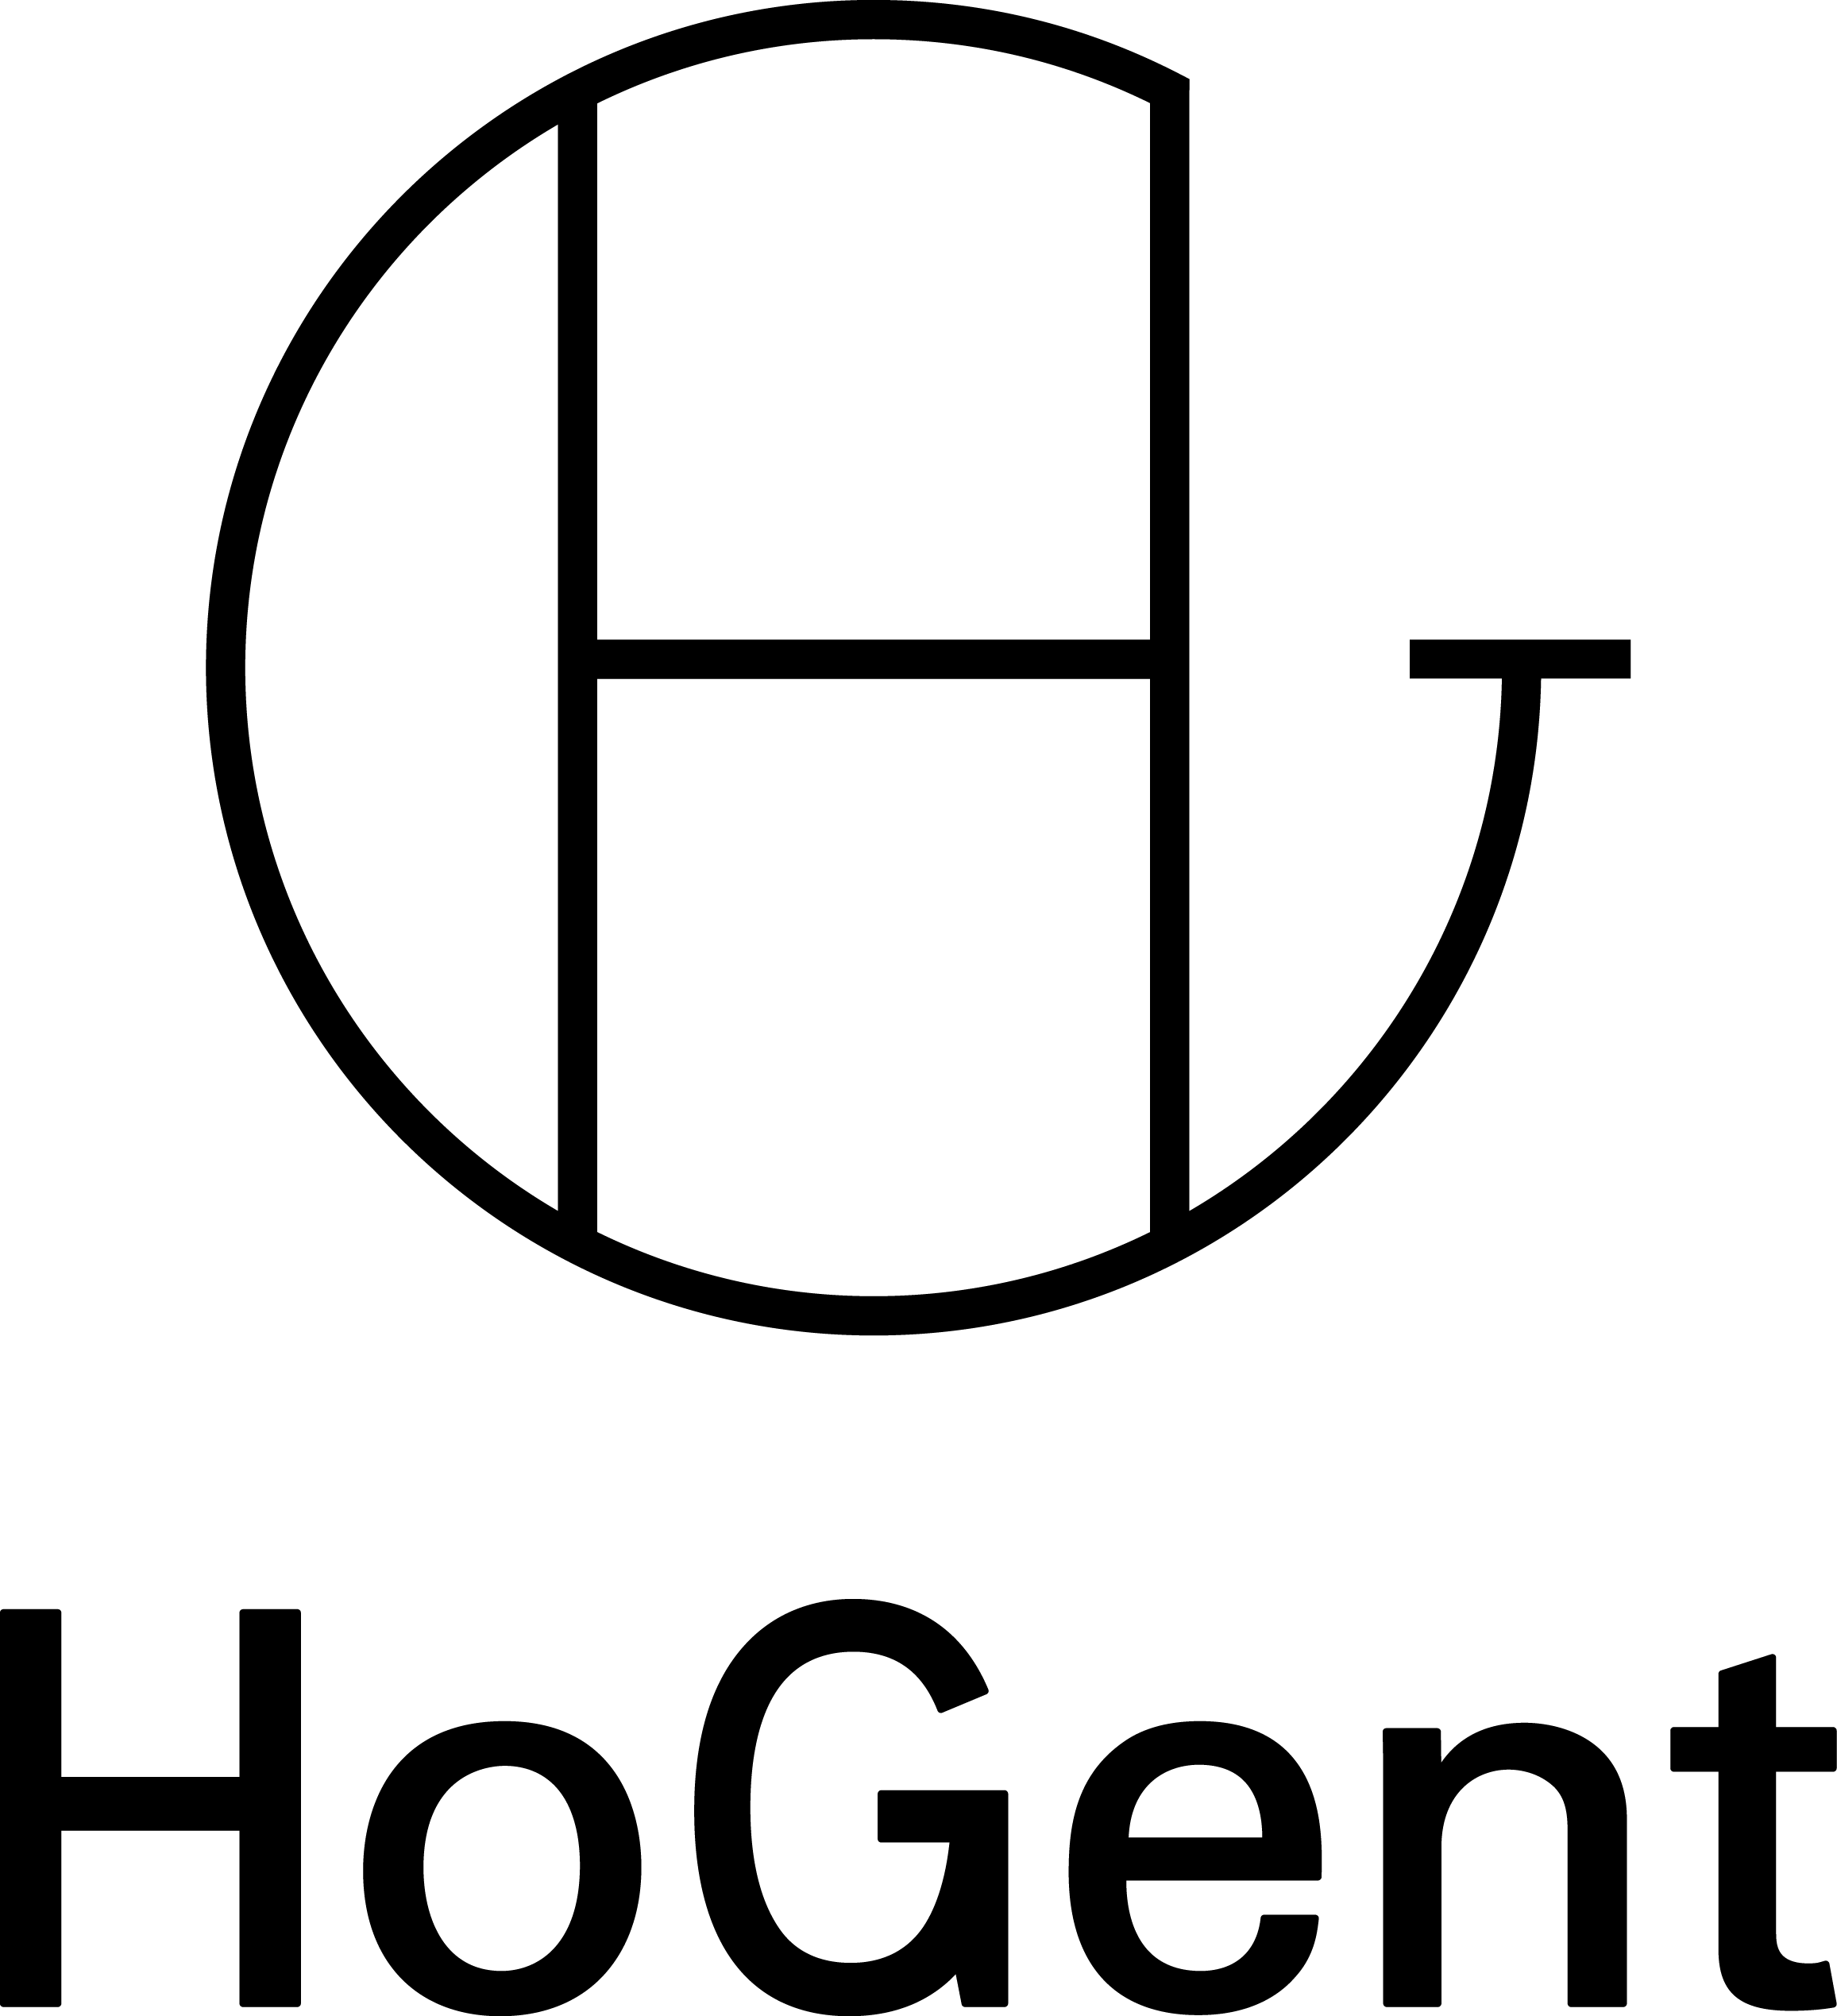
\includegraphics[width=2.5cm]{img/HG-beeldmerk-woordmerk}\\[.5cm]
    \faculteit\\[3cm]
    \titel
    \vfill
    \student\\[3.5cm]
    \rapporttype\\[2cm]
    Promotor:\\
    \promotor\\
    Co-promotor:\\
    \copromotor\\[2.5cm]
    Instelling: \instelling\\[.5cm]
    Academiejaar: \academiejaar\\[.5cm]
    \examenperiode
    \endgroup

  \end{center}
  \restoregeometry
\end{titlepage}

% Schutblad

\emptypage


\begin{titlepage}
  \newgeometry{top=5.35cm,bottom=1.5cm,left=1.5cm,right=1.5cm}
  \begin{center}

    \begingroup
    \rmfamily
    \faculteit\\[3cm]
    \titel
    \vfill
    \student\\[3.5cm]
    \rapporttype\\[2cm]
    Promotor:\\
    \promotor\\
    Co-promotor:\\
    \copromotor\\[2.5cm]
    Instelling: \instelling\\[.5cm]
    Academiejaar: \academiejaar\\[.5cm]
    \examenperiode
    \endgroup

  \end{center}
  \restoregeometry
\end{titlepage}


\begin{abstract}
% TODO: De "abstract" of samenvatting is een kernachtige (max 1 blz. voor een
% thesis) synthese van het document. In ons geval beschrijf je kort de
% probleemstelling en de context, de onderzoeksvragen, de aanpak en de
% resultaten.

Binnen de sector \gls{esports} en gaming is \gls{cheat}ing een van de grootste opkomende problemen. De gamewereld is een groeiende sector waarbij er meer en meer geld mee valt te verdienen. Er zijn toernooien voor \gls{esports} games met prijzenpotten oplopend tot 18 miljoen euro.\citep{dota2theinternational} Dit is vaak ook een van de redenen waardoor er ook vaker wordt valsgespeeld. De spelers kunnen een onfair voordeel halen dat heel miniem kan zijn tot spelbrekend aan de hand van verschillende \gls{cheat}s. De bedoeling is dan ook om dit tegen te gaan en een competitie die gespeeld wordt te controleren op eerlijkheid via ''\gls{anti}ing''.
\\

In dit onderzoek gaan we op zoek naar de populairste methodes om vals te spelen: hoe deze werken, wat de verschillen zijn en  een vergelijking van functionaliteit. 
Daarna nemen we een kijkje naar beste manieren die relatief eenvoudig te implementeren zijn om dit tegen te gaan. Deze zullen getest worden aan de hand van meerdere \gls{cheat}s die er op los gelaten zullen worden.
\\

Dit zal gedaan worden aan de hand van het zoeken van enkele veelgebruikte \gls{cheat}s. Deze worden dan getest op een server die verschillende methodes van \gls{anti}ing zal implementeren.
\\

Als laatste onderdeel wordt de mening gegeven van iemand die een stuk diepere vakkennis heeft rond dit onderwerp. De persoon in kwestie is niet direct gecontacteerd geweest maar heeft wel een onderbouwde opinie geschreven over het onderwerp die goed aansluit op het onderzoek. Dit kan ons nog verder helpen om een beter begrip te hebben van wat er zich nu precies afspeelt binnen de \gls{esports} scene.
  
\end{abstract}

\chapter*{Voorwoord}
\label{ch:voorwoord}

% TODO: Vergeet ook niet te bedanken wie je geholpen/gesteund/... heeft

De reden waarom ik dit onderzoek doe is omdat het spel \gls{csglobal} me heel hard interesseert en meer bepaald de \gls{esports} scene hier rond. Door mijn stage bij BeSports leek er nood aan iets van \gls{anti}ing, iets wat ik merkte door zo dicht tegen de spelers te staan. Zelf merkte ik ook dat er vaker valsgespeeld werd in mijn spel naar voorkeur. Dus dit onderzoek wordt gewijd aan het feit dat ik voor zoveel mogelijk spelers een toffe ervaring wil bieden.
\\

Deze bachelorproef wordt geschreven voor het beëindigen van mijn studies aan Hogeschool Gent. Dit voor het voltooien van de Bachelor Toegepaste Informatica met specialisatie in Netwerken en Besturingssystemen. Dit onderzoek vond plaats van januari 2016 tot en met mei 2016. Alles die hier in vermeld wordt zal hoofdzakelijk een momentopname zijn maar zal wel een goede indicatie zijn voor de situatie ook voor de komende tijd hierna.
\\

Ik wil BeSports bedanken voor het gebruik van de gameservers om testen op uit te voeren, dit onderzoek was zonder server niet mogelijk geweest. Ook aan de verschillende communityleden van hun platform voor het doorgeven van enkel websites met \gls{cheat} software. Als laatste wil ik ook nog Stefanie Geldof bedanken om samen testen uit te voeren op de gameservers.
\\

Ik wens u veel leesplezier toe.

\tableofcontents

% Als je een lijst van afkortingen of termen wil toevoegen, dan hoort die
% hier thuis. Gebruik bijvoorbeeld de ``glossaries'' package.
\printglossary
%%---------- Kern --------------------------------------------------------

\chapter{Inleiding}
\label{ch:inleiding}

De bachelorproef speelt zich af binnen de \gls{esports} scene. \gls{esports} staat voor ''electronic sports'' \citep{BenDirs2015}. Dit is een overkoepelende term voor alles dat met competitief gamen te maken heeft. Het kan vrij letterlijk gezien worden als een sport maar dan achter een computerscherm. Net als gewone professionele sporters hebben eSporters een strak trainingsschema die tot wel meer dan 12u per dag tijd in neemt. Wanneer er toernooien gespeeld worden valt er voor de spelers tot wel 18 miljoen dollar aan prijzengeld te winnen. \citep{dota2theinternational} 
\\

Wat \gls{esports} ook zo kenmerkend maakt is dat het vrij nieuw is maar toch al heel veel mensen aantrekt. Het platform bij uitstek om \gls{esports} te volgen is ''\gls{twitch}.tv'', hiermee kunnen mensen matchen, toernooien maar ook individuen bekijken die aan het gamen zijn. Op bepaalde momenten kunnen er tot wel enkele miljoenen mensen gelijktijdig kijken naar de grootste competities ter wereld op het vlak van gaming. Gemiddeld zijn er 500.000 mensen aan het kijken naar wat er zoal gespeeld wordt door andere mensen voor een totaal van 241.441.823.059 minuten bekeken beeldmateriaal over het jaar 2015. \citep{twitchinfographic}
\newpage

\begin{figure}[H]
\centering
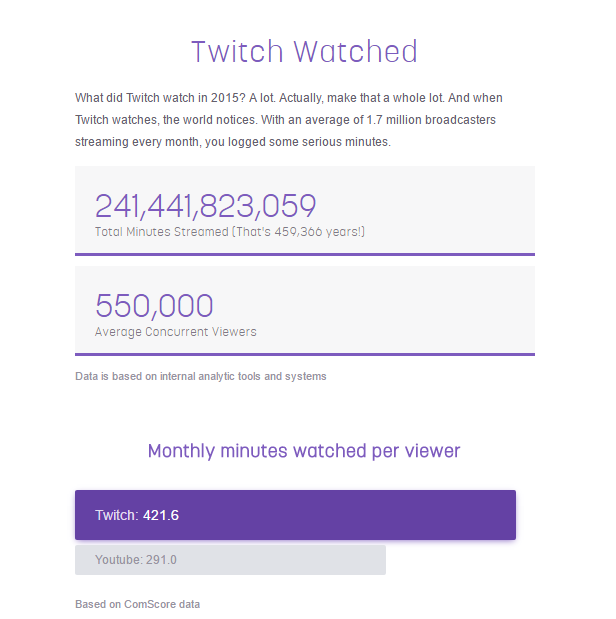
\includegraphics[width=14cm]{img/TwitchInfographic}
\caption{Aantal uren bekeken beelden op \gls{twitch}.tv}
\end{figure}  


Het genre game waar deze thesis zich op zal specialiseren zijn ''\gls{fpsgames}''. Dit staat voor First Person Shooters of met andere woorden, games waarbij mensen zich in een bepaald personage wagen en uit het standpunt van die persoon kijken. De grootste game die momenteel competitief gespeeld wordt in de \gls{esports} scene (onder de categorie \gls{fpsgames}) is de alom bekende \gls{csglobal}. 
 Met een 10 miljoen unieke spelers per maand heeft dit spel een heel grote spelersbasis en spelers van overal ter wereld. Dit is een van de meest bekeken games op \gls{twitch} en is ook een van de eenvoudigste games om te snappen vergeleken met de andere populaire \gls{esports} games. \citep{csgoblog}
\\

Het nadeel aan deze game is het grote aantal valsspelers of ''\gls{cheat}ers''. Veel spelers zijn snel geneigd om een van de veelvuldige \gls{cheat}s te downloaden en deze even te proberen wanneer ze een minder moment hebben. Het is dan ook helemaal niet moeilijk om deze te vinden na wat zoeken op het internet. Na even zoeken komen we al heel wat verschillende online fora tegen die gratis \gls{cheat}s aanbieden.
\\

websites zoals: 
\begin{itemize}
\item unknowcheats
\item MPGH: multiplayer game hacking
\item x22 cheats 
\item deadc0deshop
\item en meer
\\
\end{itemize}


 Mensen downloaden deze dan even naar hen pc en schakelen deze dan in om voordelen te krijgen op het vlak van ''\gls{aim}'' - het mikken met een geweer - of op vlak van ''pressence'' - mensen zien terwijl deze zich achter een muur bevinden (ook wel wallhack genoemd). Daarna gaat dit nog veel verder tot zelf de kleinste dingen zoals het rondspringen waardoor je meer snelheid haalt - bunnyhoppen genaamd -, dit is normaal gezien iets wat heel veel oefening bevat en zelf de beste spelers niet consistent kunnen doen. 
\\

Voor dit onderzoek zal er vooral geconcentreerd worden op het spel Counter-Strike omdat dit het meest gekend is en er dus ook het diepst op ingegaan kan worden. Andere games zijn vaak maar op kortere termijn populair. \gls{csglobal} bestaat nu al een 4 jaar maar blijft maar groeien, waartegen andere spellen dan eerder hun piek hebben bij release van het spel en dan uiteindelijk qua spelers afnemen. De technieken om vals te spelen en dit tegen te gaan zijn vrij gelijklopend tussen verschillende \gls{fpsgames} zoals Counter-Strike, Battlefield, Call of Duty... De technieken die in dit document besproken worden zullen dan ook voor andere games vrij gelijklopend zijn.
\\

\newpage

\begin{figure}[H]
\centering
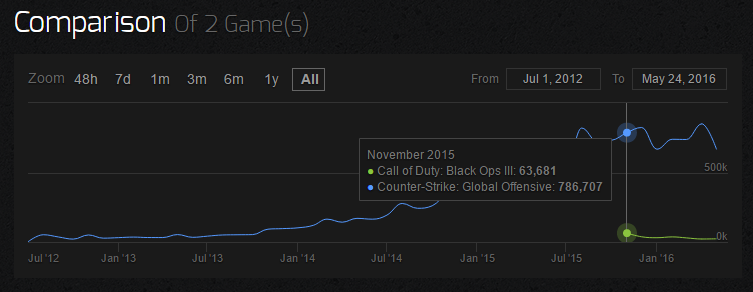
\includegraphics[width=15cm]{img/csgovsbo3}
\caption{Vergelijking van \gls{csglobal} met een Call of Duty die ongeveer in de gelijke periode geïntroduceerd is. Deze grafiek heeft het aantal spelers weer voor een bepaalde periode. Het valt op dat Call of Duty zijn spelers al weer zo goed als onbestaande zijn, dit komt ook gedeeltelijk door het jaarlijks uitkomen van een nieuw spel binnen die reeks. \citep{steamcharts}}
\end{figure} 

De reden dat we deze valsspelers uit het spel willen halen bestaat uit verschillende aspecten. Eerst en vooral het meest logische aspect: het moet voor de andere spelers tof blijven en iedereen moet op gelijke voet staan. Ten tweede hebben we dan ook het aspect qua toernooien en wedstrijden. Wanneer er geld mee te winnen valt of er staat heel wat reputatie op het spel wil je niet dat er een bepaald team of speler een voordeel heeft door het valsspelen, net zoals in andere sporten zoals voetbal bijvoorbeeld. Het zou ook voor de kijker het spannende uit het spel wegnemen.
\\ 

Eerst en vooral zal er worden uitgelegd wat nodig is te weten om het spel te snappen. Daarna zullen we de veelvuldige valsspeel manieren en tools om dit tegen te gaan bekijken.


\section{Probleemstelling en onderzoeksvragen}
\label{sec:onderzoeksvragen}
% TODO: Wees zo concreet mogelijk bij het formuleren van je
% onderzoeksvra(a)g(en). Een onderzoeksvraag is trouwens iets waar nog
% niemand op dit moment een antwoord heeft (voor zover je kan nagaan).

Voor dit onderzoek gaan we dus op zoek naar een oplossing om \gls{cheat}ers tegen te gaan binnen \gls{fpsgames} toegepast op Counter-Strike. Dit met de bedoeling om op een online platform te implementeren zodat competities binnen games zo eerlijk mogelijk kunnen verlopen. Wat is de beste en meest praktische oplossing voor deze use case. 
\\

De vragen die we willen beantwoorden bestaan uit volgende onderdelen.
\begin{itemize}
\item Waarom is het zo moeilijk om dit tegen te gaan en valt er iets te doen naast \gls{anti}ing om dit tegen te gaan.
\item Wat is de beste oplossing om aan \gls{anti}ing te doen.
\item Wat zijn de bestaande soorten \gls{cheat}s momenteel. 
\end{itemize}


\subsection{Voorbeeld uit het echte leven}
\label{subsec:voorbeeld}

Om een idee te geven hoe het probleem zich voordoet in het echte leven ga ik even in de tijd terug naar eind 2014. Op het moment dat veel mensen geïnteresseerd raakten in de game kwam er plots een \gls{cheat} schandaal naar buiten die enkele spelers aanduidde als hackers. Door een update aan het \gls{valve} \gls{anti} (VAC)systeem werden enkele \gls{cheat}s die tot toen nog niet gedetecteerd werden wel gedetecteerd waardoor er dus heel wat spelers (naast de professionele spelers) van het spel verwijderd werden. Dit moment noemt men ook wel een \gls{vac}-wave.
\\

De speler die verbannen werd was Hovik "KQLY'' Tovmassian. Op dat moment speelde deze fransman in een team samen met een van de twee Belgen die op dat moment professioneel spelen. Naast hem waren er nog twee spelers die op hetzelfde moment ook een \gls{vac}-ban toegewezen kregen. Dit is een van de meest ophef makende gebeurtenissen in de geschiedenis van Counter-Strike. Hierna werd er heel veel gezocht door andere professionele spelers maar ook door kijkers naar nog mensen waarvan het mogelijk zou zijn dat ze valsspelen. Dit zorgde voor veel problemen omdat er vaak wat spelers onschuldig beschuldigd werden waardoor er heel veel onduidelijkheid was.\citep{pcgamerhackingscandal}
\\

Het meest opmerkelijke was dan nog wel dat het moment dat deze speler zijn ban kreeg zijn team net zou vertrekken naar een van de grootste toernooien van het jaar. Het team werd automatisch de toegang ontzegd tot het toernooi en konden dus niet meedoen. Door al deze problemen is het team uiteindelijk stuk gegaan omdat de eigenaar geen sponsors meer kon krijgen door de slechte naam die zij gekregen hadden. \citep{titan}
\\

Je ziet dat een kleine slechte keuze grote gevolgen kan hebben, daarom dat het noodzakelijk is om de mogelijkheid tot valsspelen zoveel mogelijk weg te nemen zodat dit veel minder tot niet voorkomt.

\chapter{Methodologie}
\label{ch:methodologie}
Voor we aan dit onderzoek beginnen wordt aan de lezer de basis uitgelegd van wat het spel Counter-Strike nu precies allemaal inhoudt. Om ieder aspect van het onderzoek te begrijpen is deze basis nodig.
\\

Mijn testopstelling voor het controleren welke opties de beste zijn bestaat uit verschillende onderdelen. 
\\

Eerst en vooral werd het spel \gls{csglobal} tweemaal aangekocht met het vooruitzicht op gebanned te worden op deze twee accounts. Deze loggen in op een oude laptop (niet in een virtuele machine omdat er nood is aan volledige onafhankelijkheid van de tester zijn dagdagelijkse hardware en de volledige sterkte van de grafische kaart) waar het spel Counter-Strike op geïnstalleerd wordt. 

Vervolgens wordt er gezocht naar de verschillende soorten \gls{cheat}s die gebruikt kunnen worden met de laatste update van de game. Dit zijn dingen die vaak veranderen dus dit onderzoek is dan ook enkel van toepassing op het moment van schrijven, het kan zijn dat dit na een maand anders is.
\\

In dit onderzoek wordt eerst een grondige uitleg gegeven wat de game Counter-Strike precies inhoudt. Het is moeilijk om ieder aspect van het onderzoek te snappen zonder dat de basis van het spel duidelijk is. Hierna wordt er eerst dieper ingegaan op de verschillende soorten \gls{cheat}s en wat meer over de werking hiervan. Vervolgens wordt er gekeken welke precieze manieren er zijn om dit tegen te gaan. Dit is opgedeeld in twee hoofdcategorieën: eerst de softwaretools die vaak beter gekend zijn, daarna wat meer over een nieuwe oplossing met hardware. 

\newpage
Als laatste is het de bedoeling om een testopstelling te maken die op de servers test welke \gls{cheat}s gevangen worden door welke \gls{anti}s. Er wordt dan gekeken welke opties de beste oplossing biedt en of er een combinatie mogelijk is om zo veel mogelijk valsspelers tegen te gaan. 


\chapter{Counter-Strike: Global Offensive}
\label{ch:csgo}
Voor we beginnen aan het onderzoek naar verschillende manieren om vals te spelen en om deze tegen te gaan moeten we eerst de basis van het spel snappen. In dit onderzoek gaat het om het spel \gls{csglobal} of kort ''CS:GO''. Deze game is een van de meest gespeelde competitieve games en staat er voor gekend om eenvoudig aan te leren zijn vergeleken met andere competitieve \gls{esports} games. 
\\

De voorganger van deze immens populaire game werd uitgebracht op 19 juni 1999. Origineel was dit een modificatie voor de uiteengezette en beruchte game "Half-Life". Er zijn heel wat games die vandaag de dag als alleenstaande verkocht worden die ooit begonnen zijn als een speltype gemaakt door spelers die bouwden op de basis van Half-Life. Na deze mod heeft \gls{valve} (de huidige ontwikkelaar achter Counter-Strike en Half-Life) een samenwerking met deze spelers aangekondigd en kon de game als alleenstaand spel gespeeld worden.
\\

Na vele bèta's en heel wat patches werd de final versie gereleased. Deze release is een van de bekendste bij het competitieve onderdeel van Counter-Strike, deze staat gekend als "1.6". Dit werd snel een van de meest populaire competitieve computer games ooit en werd tot voor kort nog altijd gespeeld door veel professionele gamers hoewel deze toch al wat leeftijd had.
\citep{dusttodust}
\\

Hierna kwamen nog een andere versie genaamd ''Counter-Strike: Source''. Hoewel deze ook heel wat verkoop had is deze minder gespeeld geweest. De game waar wij ons op zullen concentreren is de in 2012 geïntroduceerde ''\gls{csglobal}''. Deze versie van het spel is deze die vandaag de dag nog altijd gebruikt wordt in de competitieve wereld.

\begin{figure}[H]
\centering
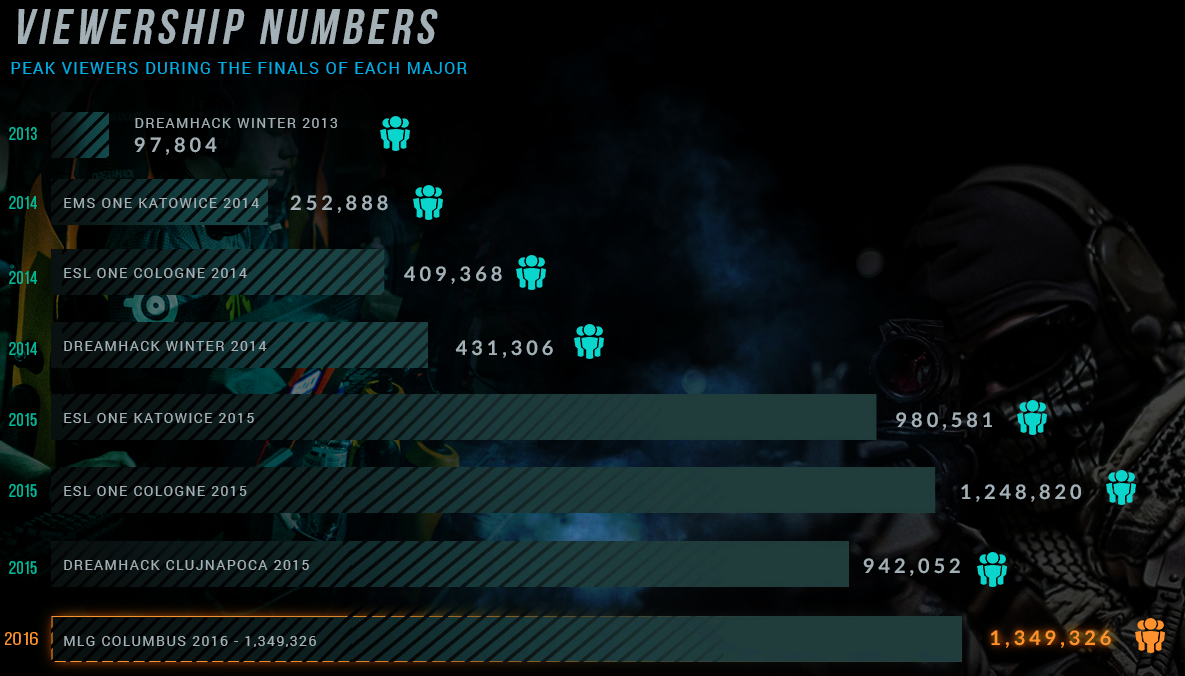
\includegraphics[width=15cm]{img/dathostInfographic}
\caption{Stijging in populariteit van de game CS:GO (aantal kijkers op de grootste toernooien over de laatste jaren)}
\end{figure}

\section{Algemeen doel van het spel}
\label{sec:algemeen doel van het spel}
Counter-Strike is niet zoals de meeste andere \gls{fpsgames}. Waar bij vele shooter games het vooral gaat om het gewoon neerschieten van de tegenstander en het aantal ''kills'' of ''deaths'' telt is dit bij Counter-Strike toch nog goed anders.
\\

Bij Counter-Strike spelen er vijf spelers in twee teams, deze teams kunnen ofwel ''\gls{CT}'' (of CT) ofwel ''\gls{T}'' (of T) zijn. Elk team heeft zijn eigen doel doorheen het spel. Heel eenvoudig kunnen we zeggen dat de \gls{T}s als doel hebben ofwel de ene bom die ze hebben tot ontploffing te brengen, ofwel door alle \gls{CT}s te doden. 
De \gls{CT}s daarentegen hebben dan als doel ofwel de bom onschadelijk te maken (als deze geplaatst werd) of om alle \gls{T}s te doden. Dit wordt herhaald tot een maximaal van 30 ronden die elk een tweetal minuten duren (afhankelijk van of de bom g. Aan 15 ronden (of halverwege het spel) worden de teams omgewisseld van kant, de \gls{CT}s worden dan de \gls{T} en omgekeerd. Het eerste team dat 16 ronden wint in totaal wordt de winnaar van de game gezien.
\\

Een game wordt gespeeld op een bepaalde ''\gls{map}'' of kaart. Deze bevat een locatie waar de \gls{T} bij het begin van de ronde starten -\gls{T}s \gls{spawn}- en een waar de CT's \gls{spawn}en. Naast dit zijn er nog twee locaties waar de bom geplaatst kan worden per kaart, dit zijnde: bomb site A en bomb site B. Daar kunnen ze binnen een bepaald afgebakend gebied de bom plaatsen om daarna de komst van de CT's af te wachten. Iedere \gls{map} heeft ook unieke eigenschappen en maakt het daardoor vaak iets voordeliger om te starten aan een specifieke kant.
\\

Dit klinkt nog allemaal niet zo moeilijk tot nu toe maar buiten deze regels heb je nog het geld die iedere speler heeft. Ieder team begint de eerste ronde met \$800 en kan daarmee kiezen om iets te kopen van wapen of iets van ''utility'' of ''gear'' zoals een ''defuse kit'' (hiermee kan wordt de tijd voor het onschadelijk maken van de bom gehalveerd van 10 naar 5 seconden) of een kevlar vest waardoor je minder schade krijgt. 
Omdat er in de eerste ronde niet veel geld ter beschikking staat kan er niet anders gekocht worden dan een pistool en wordt deze ronde ook wel de ''pistol round'' genoemd.
\\

Iedere ronde krijgt een bepaalde speler geld voor zichzelf of voor het team aan de hand van wat er gedaan wordt. Voor een kill met een specifiek wapen komt er een bedrag bij de speler zijn pot. Hetzelfde voor het plaatsen van de bom. Maar als de ronde gewonnen wordt (bijvoorbeeld door de bom tot ontploffing te brengen) krijgt het hele team geld. Het verliezende team krijgt dit dan ook maar een heel stuk minder.
\\

Dit is een van de belangrijkste aspecten van het spel, het is heel handig als je kan inschatten of het ander team alles kan kopen die nodig is of als deze zullen moeten sparen en dan de ronde erna alles zullen kopen. Het sparen en enkel spelen met het standaard pistool wordt ook wel ''eco'' genoemd. Als je als een van de laatste spelers overblijft in je team en het ander team heeft nog alle spelers in leven zal het wapen vaak gespaard worden voor de volgende ronde, dit noemt men ook wel eens ''saven''.


\chapter{Cheats: schets van valsspeel mogelijkheden}
\label{ch:cheats}

Om te snappen hoe we het valsspelen moeten tegengaan moeten we eerst begrijpen hoe het valsspelen precies werkt. Er wordt een korte introductie gemaakt bij iedere soort en wat ze precies doen. Verder wordt er uitgelegd waarom ze precies zo vervelend zijn.
\\

De taal waarin vele \gls{cheat}s geschreven zijn is Assembly. Dit is een heel low level language. Dit gaat dus vaak inspelen op geheugen adressen en in direct contact met de CPU van een computer. Het nadeel aan deze taal is dat er vaak geen mogelijkheden aanwezig zijn die andere programmeertalen zo interessant maken zoals variabelen, overerving...
\citep{assembly}

Er zal niet gekeken worden naar packet sniffing met Wireshark en dergelijke gewoon omdat de pakketjes niet anders zijn dan gewone pakketjes. Deze worden aangepast op de client alsof deze iets doet die een gebruiker ook zou kunnen doen waarna het naar de server wordt verzonden. Dit is ook de reden waarom \gls{anti}ing ook zo moeilijk is en de reden waarom de server dit ook moeilijk kan herkennen aan de hand van de netwerk pakketten.

\section{Soorten}
\label{sec:soorten}
\section{Wallhacks}
\label{sec:walls}
De eerste onderscheiding die we maken zijn ''wallhacks''. Dit is een van de meest gebruikte termen onder spelers. Vaak wordt er op een incorrecte manier melding gemaakt van deze \gls{cheat}s omdat ze het meest gekend zijn. Maar wat is het nu precies?
\\

Als je je in het spel begeeft kun je met wallhacks heel eenvoudig iedereen zien lopen door de muur. Dit kan op verschillende manieren weergegeven worden. De eenvoudigste methode die door programmeurs gebruikt wordt is de box methode. Deze tekent rond ieder persoon een hokje die je door alle objecten in het spel kan zien. Zo kan je anticiperen waar de vijand zal verschijnen en heb je dus teveel oneerlijke informatie. 
De tweede manier die iets duidelijker te zien valt is met een outline rond de persoon die de vorm weergeeft hoe deze precies staat. Dit maakt het nog iets eenvoudiger voor de valsspeler omdat deze ook perfect weet waar de persoon zijn hoofd is, zijn armen enz. Op die manier kan je dus heel eenvoudig al op iemand zijn hoofd gaan mikken. Ook kan de visibiliteit erg verbeteren waardoor je wederom het onfair voordeel haalt.

Hieronder even de twee verschillen naast elkaar.

%SV_OCCLUDE_PLAYERS

\begin{figure}[H]
\centering
\begin{minipage}{0.48\textwidth}
\centering
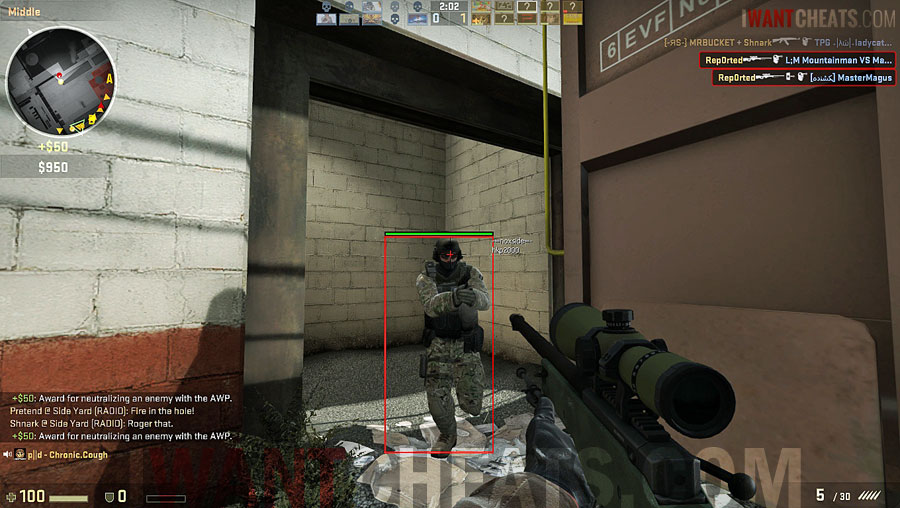
\includegraphics[width=7cm]{img/wallhack-example-box}
\caption{Wallhack met een box (merk het rode hokje op rond de persoon)}
\end{minipage}\hfill
\begin{minipage}{0.48\textwidth}
\centering
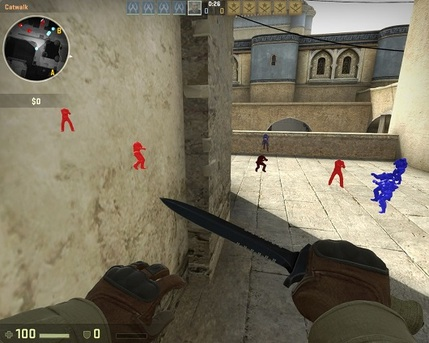
\includegraphics[width=7cm]{img/wallhack-example-outline}
\caption{wallhack met outline}
\end{minipage}
\end{figure}  

Een persoon met deze extra informatie kan op veel verschillende manier het spel beïnvloeden. Een van de eerste manieren om dit te doen is gewoon letterlijk volgen waar het andere team heengaat en anticiperen op deze situatie. Dit kan dan ook bijvoorbeeld meegedeeld worden aan een teammaat die niet aan het valsspelen is. Zo kan je als enige \gls{cheat}er heel eenvoudig het volledige spel beïnvloeden.

%(http://www.theregister.co.uk/2001/05/10/asus_releases_games_cheat_drivers/)

\subsection{Werking}
\label{subsec:werking}
Hoe is het precies mogelijk dat mensen weergegeven worden door de muur? Dat heeft te maken met de pakketten die tussen server en client worden verzonden. Iedere server verzend zijn pakketten naar de client, dit bevat de data van waar je teammates rondlopen, waar de vijand rondloopt, waar er smokes liggen en waar schoten geregistreerd zijn. De client zend zelf door wat er precies gebeurd achter de speler zijn pc. Dit zijn: waar die precies rondloopt, wanneer hij schiet en waar, welk wapen deze gebruikt en andere. Hoe de meeste gameservers werken is als volgt: alle data wordt doorgestuurd naar de client waar de onderdelen verwerkt worden. Dus de locatie van de niet zichtbare vijanden worden verzonden naar de client maar deze beslist wanneer deze weer te geven en wanneer niet.
\\

Voor \gls{cheat}ontwikkelaars is het dus zo dat zij de data die de server verzend - maar normaal niet wordt weergegeven door de client - via hun software toch wordt weergegeven. Dit dan op de verschillende manieren zoals hierboven weergegeven.
\\

Dit in Counter-Strike recent tegengegaan door de data die verzonden wordt door de server te minimaliseren. Enkel echt relevante data wordt doorgestuurd naar de client. Dus veel wallhacks werken hierdoor niet meer omdat niet alle data bij de gebruiker aanwezig is. De naam van de technologie hierachter is PVS of ''Potentially Visible Set''. Dit berekent wanneer een gebruiker een vijand kan zien en of horen en aan de hand daarvan wordt de data doorgestuurd. Op die manier is het enkel mogelijk voor \gls{cheat}s om personen weer te geven als deze ofwel door een teammaat gezien werden of wanneer je ze zelf ziet. Dit bestond al een heel stuk langer om de game te optimaliseren door te berekenen vanaf welke plaats je welke objecten kan zien maar nu wordt dit dus ook gedaan met de spelers zelf. 
\citep{PVS}
Dit is standaard ingesteld maar kan aangepast worden door op de server de server variabele SV\_OCCLUDE\_PLAYERS op 1 te plaatsen.

\section{ESP}
\label{ESP}
Als tweede \gls{cheat} hebben we ESP wat staat voor ''Extrasensory Perception''. Extrasensory perception komt uit de wereld van de telepathie, wat gedefinieerd kan worden als "the ability to know things (such as what another person is thinking or what will happen in the future) that cannot be known by normal use of the senses" \citep{extrasensoryperception}. We vermelden deze als tweede omdat ESP heel vaak wordt gebruikt in combinatie met wallhacks. Net zoals bij de telepathie geeft deze extra hulp aan de gebruiker door informatie door te geven over de vijand. Dit niet over de locatie waar deze loopt maar vaak eerder over hoeveel geld de vijand beschikt en hoeveel ''health'' een bepaalde vijand nog heeft.
Omdat dit heel 'droge' informatie is wordt dit vaak weergegeven naast een wallhack. Een voorbeeld kan je hieronder zien, let vooral duidelijk op het groene lijntje erbij. Dit is hoeveel levenspunten of ''health'' de vijand nog over heeft.

\newpage
\begin{figure}[H]
\centering
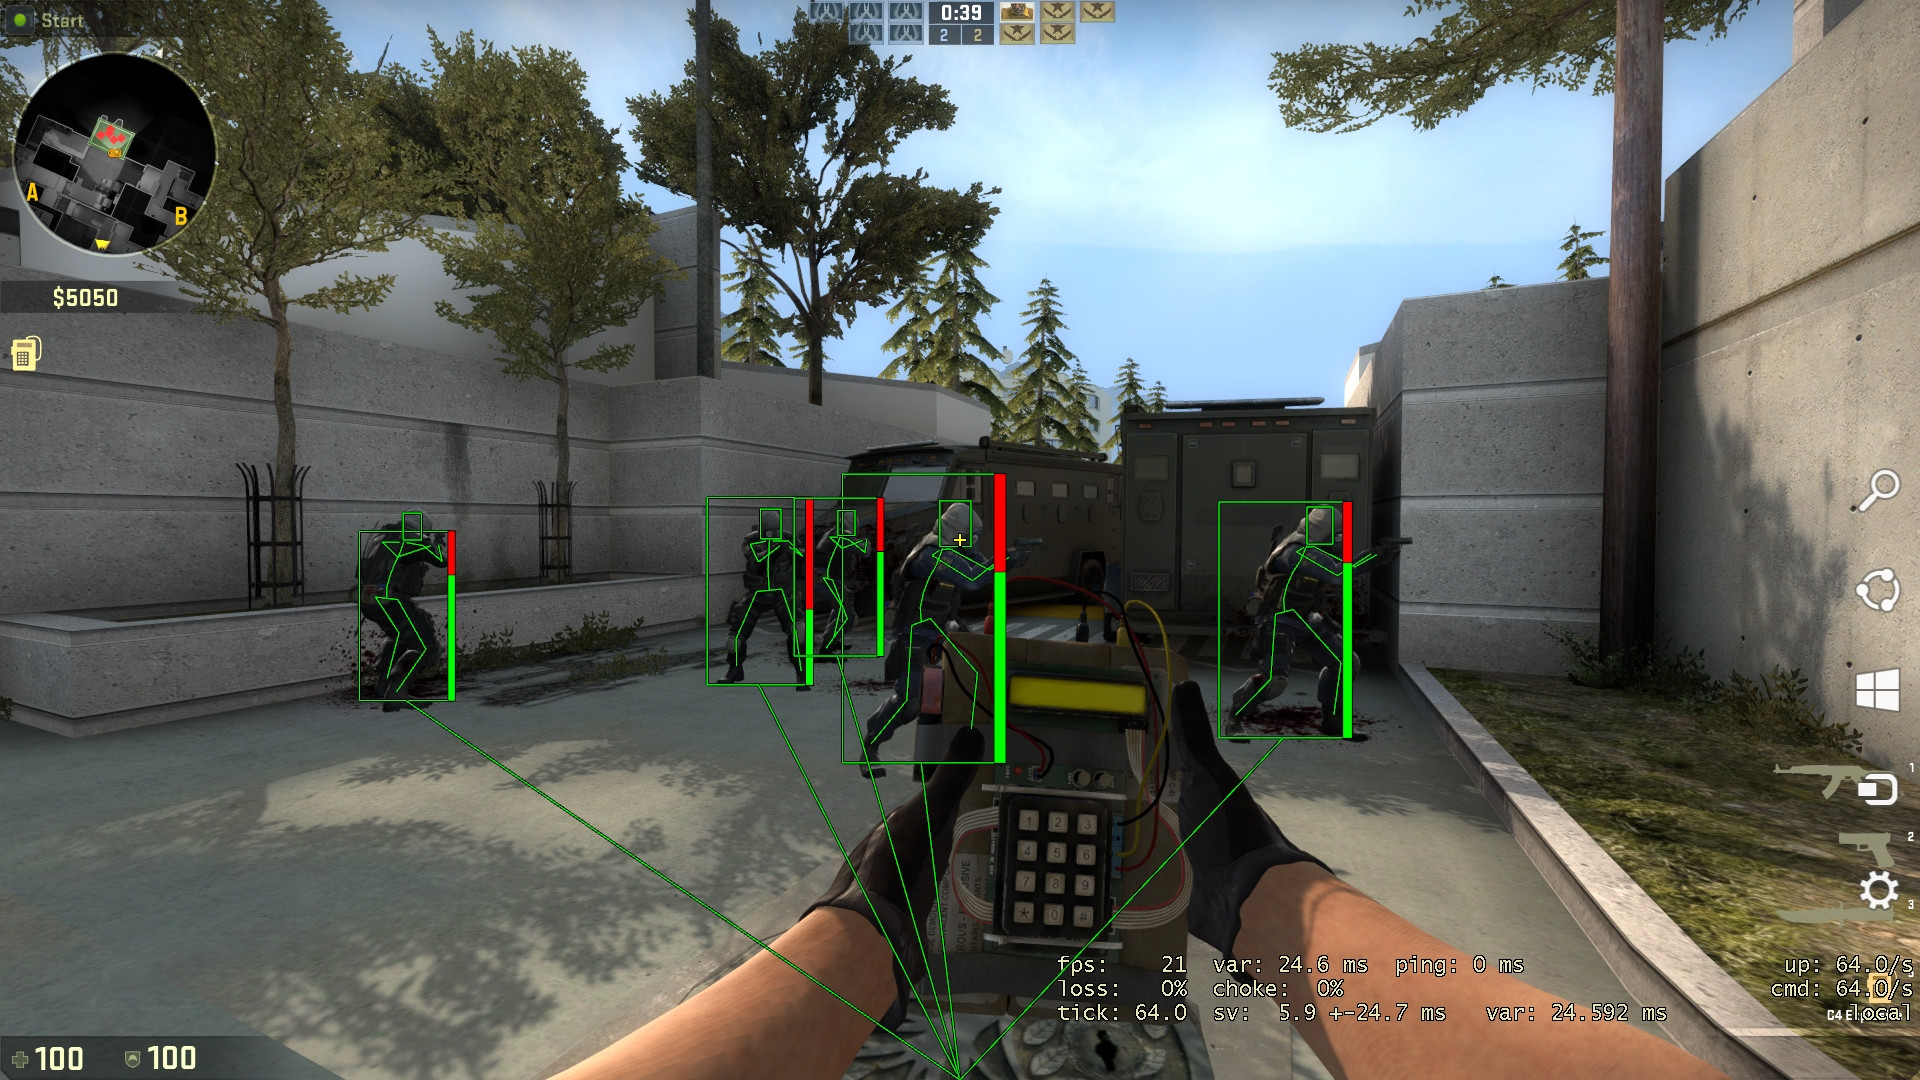
\includegraphics[width=15cm]{img/esp-example}
\caption{Wallhack in combinatie met ESP (let op het groene balkje die aanduidt hoeveel leven nog resterend is per persoon)}
\end{figure}
  
\section{Aimhacks}
\label{sec:aim}
Wat het spel Counter-Strike nu zoveel anders maakt vergeleken met andere \gls{fpsgames} is dat deze heel wat training vereist om ieder wapen te kunnen beheersen. Het is zo dat ieder wapen een bepaald uniek karakter heeft. Bij gewone geweren of ''Rifles'' is er vaak een patroon die deze volgt als je hem in een keer leegschiet, dit wordt het ''spray pattern'' genoemd. Dit is het omhoog gaan van het wapen in een bepaalde beweging wanneer je schiet. Omdat dit altijd hetzelfde is kan je ook dit tegengaan door je muis in de tegengestelde richting naar beneden en/of naar links of rechts te bewegen. Een voorbeeld van zo'n spray pattern is hieronder afgebeeld voor een van de wapens.
\\  

Het is dus mogelijk om dit tegen te gaan door in omgekeerde richting te bewegen met de muis en zo de spray te controleren. Dit is een van de \gls{cheat}s die vaak bij \gls{aim}hacks voorkomt. Zodra de gebruiker begint te schieten worden muisbewegingen gesimuleerd aan de hand van welk wapen ze precies vast hebben. Dan moet de gebruiker wel nog zelf de persoon zien te volgen natuurlijk. En dat is waar de echte \gls{aim}hacks te pas komen.

\begin{figure}[H]
\centering
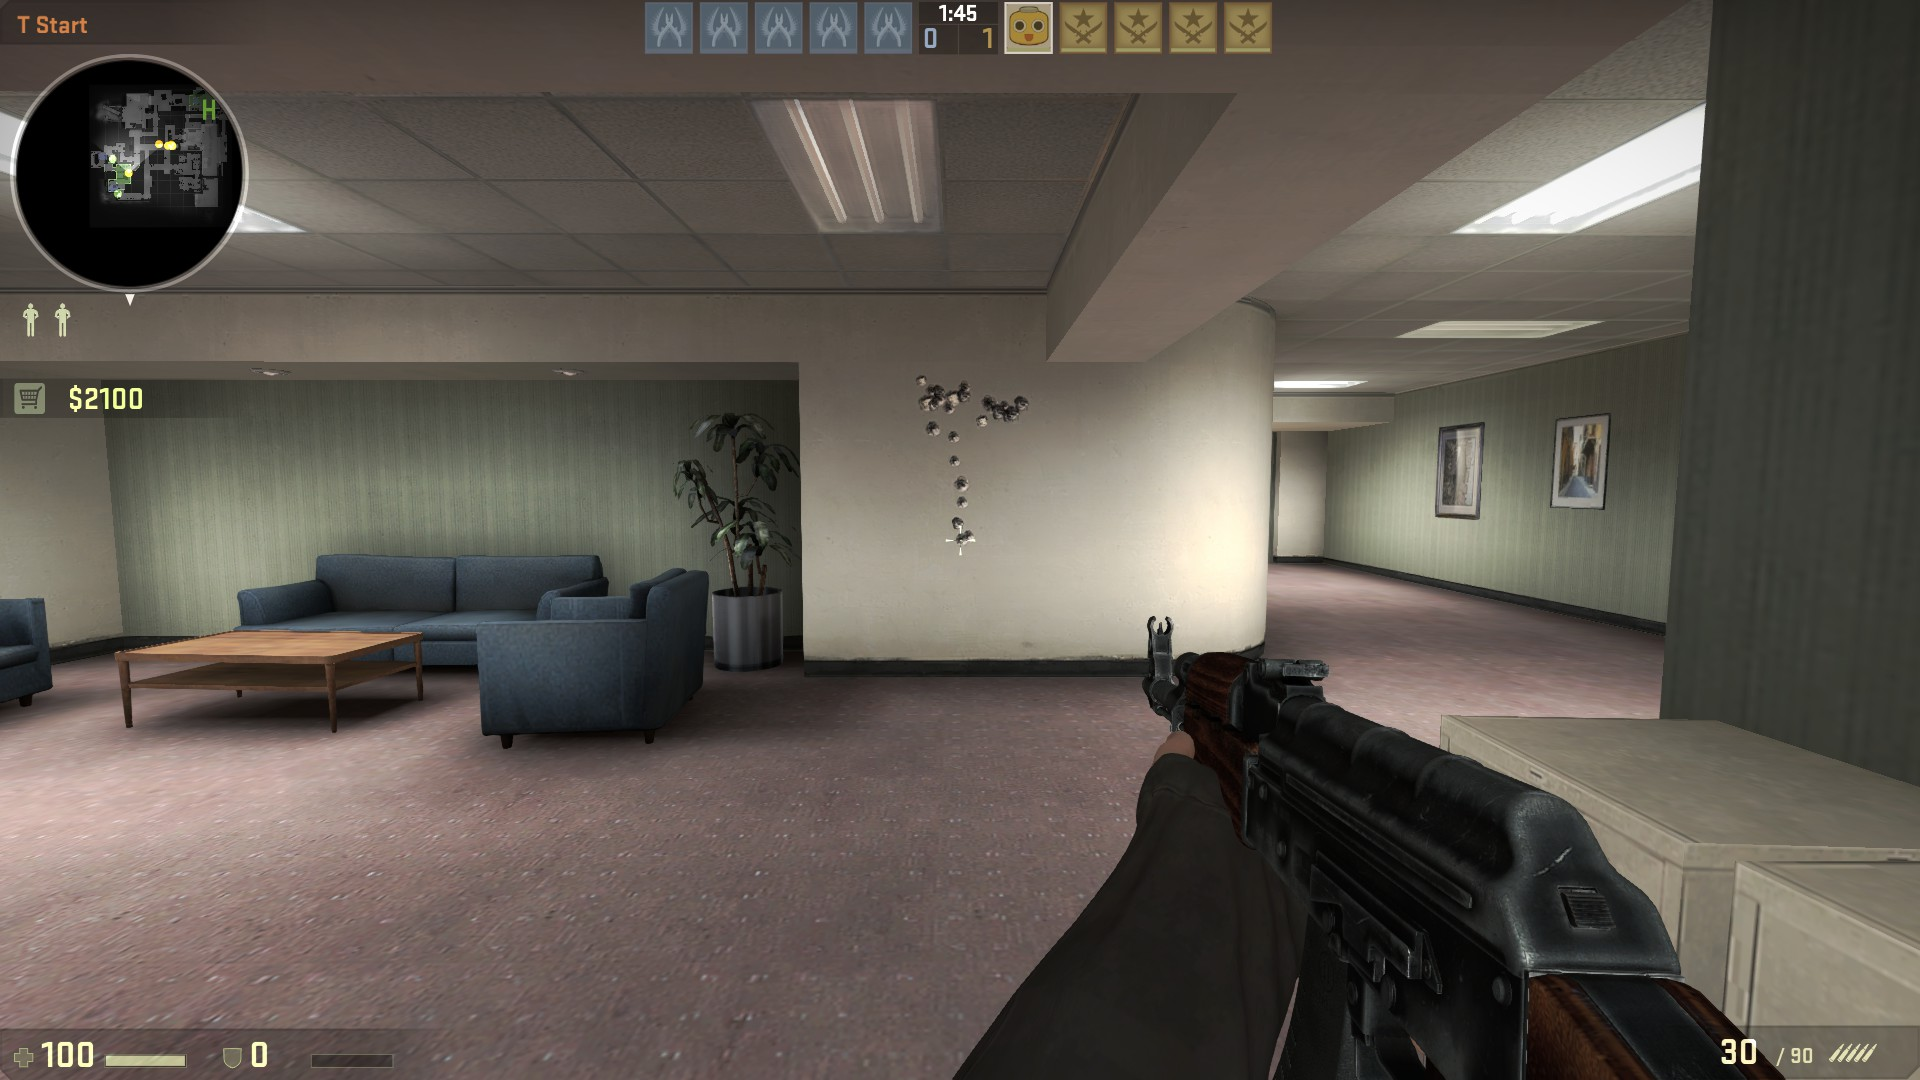
\includegraphics[width=15cm]{img/spraypattern-example}
\caption{Een spray pattern}
\end{figure}

De tweede vorm die vaker gebruikt wordt dan bovenstaande is iets moeilijker (voor de cheat ontwikkelaar) maar maakt het de speler heel eenvoudig. Deze zal voor de speler mikken op een vijand en dan nog wel liefst op het hoofd. Deze is wederom in Assembly geschreven. Een interessante reeks video's zijn deze van \cite{basicaimbottutorial}. Dit is een forum waarin de basis voor het maken wordt getoond voor het maken van een hack of \gls{cheat}. In onderstaande afbeelding kan je duidelijk zien dat er gewerkt wordt met de geheugen adressen van het systeem. 
\\

De toepassing van deze laatste verschilt wel nogal onderling tussen verschillende programma's. De ene zal automatisch door een druk op de toets een persoon volgen zonder dat jij de muis moet bewegen (wat heel hard opvalt ook). De andere soort zal dan eerder de gebruiker verder helpen als hij in de buurt komt van een speler om op het hoofd te schieten. Ze zijn beiden bijna even doeltreffend enkel is de eerste manier veel opvallender als er bijvoorbeeld meegekeken wordt naar de speler door iemand anders.
\newpage

\begin{figure}[H]
\centering
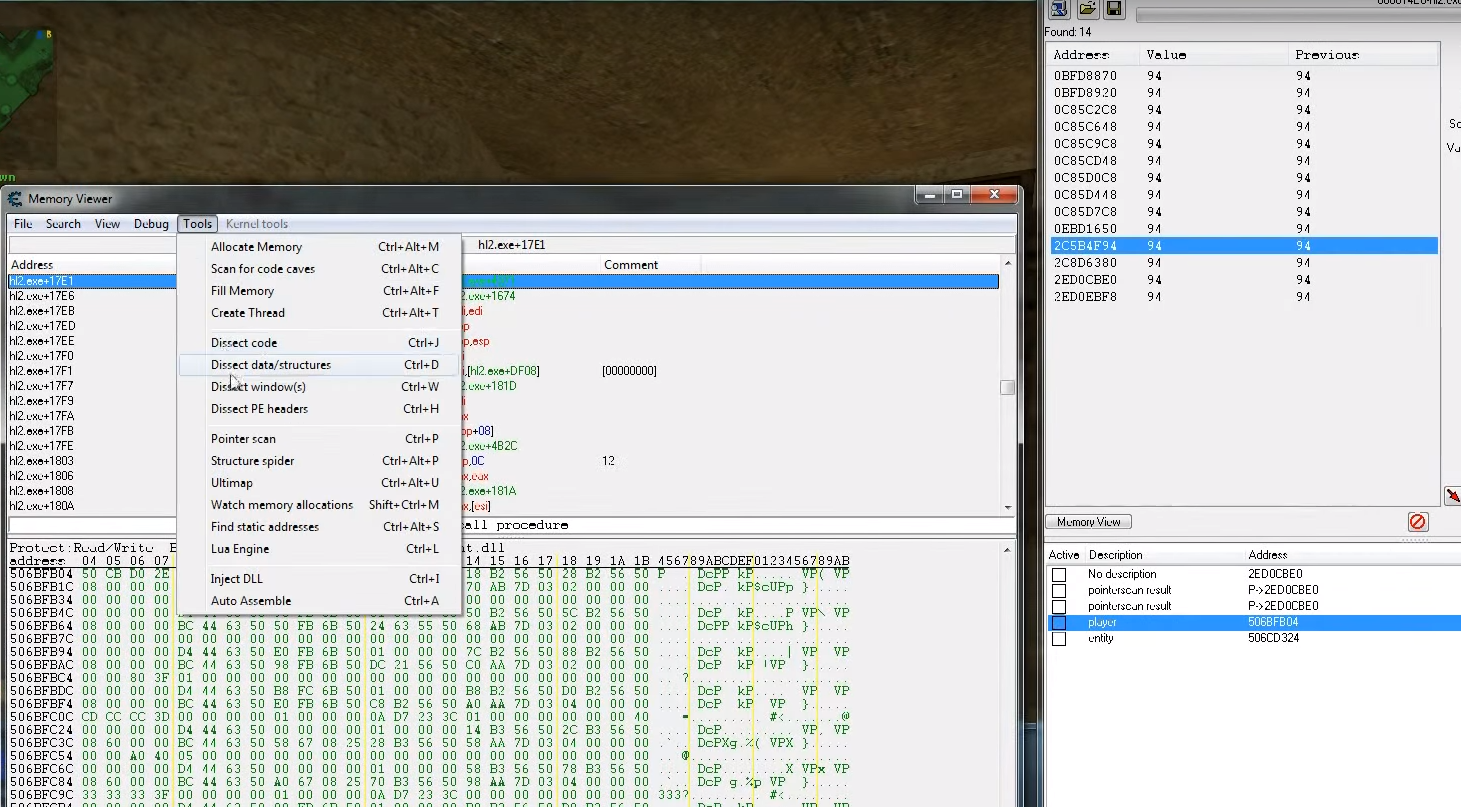
\includegraphics[width=15cm]{img/aimhack-code-example}
\caption{Een voorbeeld van de gebruikte software om de geheugenadressering aan te spreken}
\end{figure}

\section{Gebruik}
\label{sec:gebruik}
Maar hoe moeten we dit nu precies voorstellen voor de eindgebruiker? De eenvoudigste \gls{cheat}s (die vaak ook vrij snel gedetecteerd worden) zijn vaak gewoon Windows executables dus een .exe die je gewoon uitvoert. Het nadeel voor de mensen die de \gls{cheat}s uitvoeren is dat deze heel vaak eenvoudig herkenbaar zijn door \gls{anti}s omdat ze logische benamingen gebruiken, de code vaak vrij gelijkaardig is, ze altijd onder dezelfde naam uitgevoerd worden enz.
\\

Daarvoor zijn er dan ''polyhacks'' om het probleem op te lossen. Dit zijn hacks die de standaard .exe file iedere keer onder andere instellingen en een andere naam runnen. Dit maakt het ontdekken van deze een heel stuk moeilijker wat het bestrijden dus ook vaak erg moeilijk maakt voor serverbeheerders. Veel hacks werken vaak ook dan enkel op deze manier omdat deze anders te snel zouden gevangen worden door een systeem die patronen zoekt onder meerdere gebruikers. Door dit dan op hun \gls{cheat} te verplichten kan deze een heel eind langer onopgemerkt meegaan.
\newpage
Dan heb je ook nog het injecteren van een .dll bestand. Deze voeg je dan in in een programma die vaak wel als veilig wordt gezien waardoor deze vaak niet gedetecteerd wordt. 
\\

Deze twee bovenstaande methoden hebben natuurlijk enkel maar nut als het een \gls{anti} is die het bestandssysteem meescant op rare processen (zoals bijvoorbeeld deze van de grotere \gls{esports} bedrijven zoals ESEA). Veel anti-cheat software draait op de server en kan de gebruiker zijn bestanden dus niet scannen. \citep{esea}

\chapter{Anti-Cheats: Bestrijding van de valsspelers}
\label{ch:antis}
Het belangrijkste aspect van deze bachelorproef is het tegengaan van het valsspelen. Dit is waar we nu op in zullen gaan. Dit onderdeel wordt opgedeeld in 3 hoofdcategorieën. Eerst de software tools die op de gameserver draaien. Ten tweede heb je dan ook iets nieuw en opkomend: de \gls{anti} hardware. Als laatste hebben we nog de sociale of crowd-sourced \gls{anti}s.

\section{Software}
\label{sec:antisoftware}
Als eerste zullen we even de software overlopen. Dit is de meest voorkomende oplossing en heeft dus ook iets meer oplossingen ter beschikking. Omdat het belangrijk is dat \gls{anti} software mee is met de laatste vernieuwingen is er hoofdzakelijk geconcentreerd op software die nog altijd actief werkt en die ook zeker werkt voor \gls{csglobal} en niet voor de oudere versies van het spel. 

\subsection{VAC: Valve Anti-Cheat}
\label{sec:vac}
De grootste en meest bekende software is de Valve Anti-Cheat software. Dit komt standaard bij iedere installatie van de game en ook iedere server runt dit standaard wanneer deze opgestart wordt. \citep{VAC}Omdat iedere speler deze software staan heeft is dit ook de software die de meeste gebruikers pakt in absolute waarden. In totaal zijn er bijna een vier miljoen bans uitgedeeld tot op dag van vandaag. Dit is dan ook het voordeel aan dit stuk software, iedere gebruiker draait het onzichtbaar ook op zijn PC, dit is niet uit te schakelen als je aan officiële matchen wil meedoen.
\citep{steamdb}
\\

Hoewel dit heel doeltreffend is kan er toch nog veel beter ontwikkelt worden aan deze technologie. Zoals je in mijn voorbeeld uit het echte leven kan lezen is dat er af en toe toch nog mensen voor langere tijd niet gedetecteerd worden. Zelf professionele spelers dus. Er kan dus zeker nog wel heel wat verbetert worden aan deze technologie. 
\\

Hoewel dit \gls{vac} in een negatief beeld plaats wordt er wel nog actief ontwikkelt en zijn er vaak wat ze noemen ''\gls{vac} Waves''. Dit zijn momenten wanneer er een hele hoop personen in een keer verbannen worden. Dit is vaak door een update (die niet zichtbaar is voor de speler) van de tool. 
\begin{figure}[H]
\centering
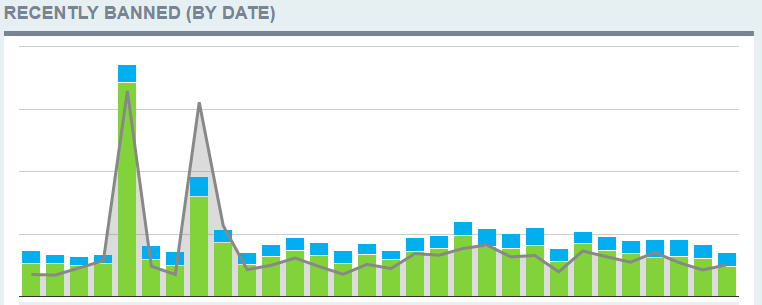
\includegraphics[width=15cm]{img/banwave}
\caption{Volgende grafiek toont het aantal verbannen personen door \gls{vac} per dag. Let op de pieken,dit zijn ''\gls{vac} Waves''. \citep{vacbans} }
\end{figure}

Dus als serveradministrator wordt er vaak gekozen voor een third-party tool die dit moet tegengaan. Deze zijn vaak nog een heel stuk diepgaander en beter uitgewerkt. Het enige nadeel hiervan is dat deze ook genoeg moeten geüpdatet zijn om hedendaags te gebruiken.


\subsection{Sourcemod}
\label{sec:sourcemod}
Een van de belangrijkste tools die nodig is om geavanceerde wijzigingen door te voeren op een gameserver met de Source engine (de game engine van \gls{valve} en waar Counter-Strike op draait) zijn plugins en meer bepaald Sourcemod. Deze biedt nog veel meer functionaliteit aan dan anders mogelijk zou zijn. Standaard bevindt er zich functionaliteit in om plugins te runnen. Sourcemod is zo'n gewone plugin die veel geavanceerdere plugins mogelijk maakt die dan draaien onder Sourcemod. Er zijn dan heel wat software pakketten die deze gebruiken om hun functionaliteit doeltreffender te maken. 
\\

Sourcemod is heel eenvoudig zelf te installeren. Men download de benodigde files plaatst deze via FTP op de gameserver in de juiste \gls{map} en herstart de gameserver. Nadien kun je via commando's nagaan of dit correct werkt. Eenmaal dit correct is ingesteld is het eenvoudig om modificaties toe te voegen zoals bijvoorbeeld een \gls{anti}. \citep{sourcemod}

\subsection{SMAC: Sourcemod Anti-Cheat}
\label{sec:smac}

Sourcemod Anti-Cheat is een van de weinige \gls{anti}s die open source is en nog actief door de community ondersteund wordt. Zoals de naam het al zegt is deze een volledige plugin in Sourcemod. De code is gebaseerd op een andere \gls{anti} die tegenwoordig niet meer verkrijgbaar is genaamd Kigen \gls{anti}. Het probleem hierbij is dat de laatstgenoemde een copyright claim hebben ingediend waardoor \gls{smac} niet meer openlijk mag verdeeld worden. Na wat zoeken kwam ik dan toch terecht op de laatst gepubliceerde versie.\citep{smac}
\\

Deze \gls{anti} is een van de meest bekende omdat deze voor een groot online platform genaamd FaceIT gebruikt werd. Nu hebben ze hun eigen herwerkte versie van \gls{smac} die ook met heuristische berekeningen werken.

Dit is een van de \gls{anti}s die het uitgebreidst zal getest worden omdat deze gratis beschikbaar is voor iedereen.

Nog een voordeel van deze is dat deze ook rekening kan houden met globale lijsten van gebande spelers. Dit maakt het een heel interessante optie want wanneer er iemand \gls{cheat} op een andere server (mogelijks zelf met een andere \gls{anti}) wordt deze toch gebanned van u server.

Over deze banlists straks meer.

\subsection{Easy Anti-Cheat}
\label{sec:easy}
Easy \gls{anti} is een van de betaalde opties onder de mogelijke oplossingen. Zij bieden op hun website een optie aan voor \gls{esports} die een server - client oplossing heeft. Dit houdt in dat de gebruiker voor hij de server kan joinen een programmatje moet downloaden die daarna data terugzend naar de \gls{anti} server die bij het bedrijf onderhouden wordt. Het voordeel hieraan is dat je heel weinig administratie werk hebt maar het nadeel is dat je niet weet wat er gebeurt met de data van je spelers.

Ook met de module van \gls{smac} die spelers banned die al gebanned zijn van Easy \gls{anti} lijkt me het onnodig om te betalen voor deze software. Natuurlijk moeten je spelers dan wel al eens gespeeld hebben op een server die deze software draaiende had.\citep{eac}

\begin{figure}[H]
\centering
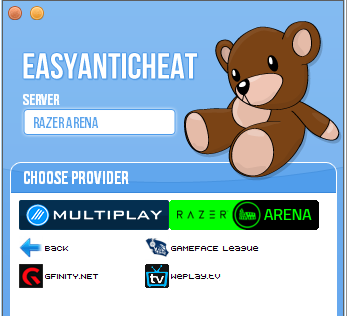
\includegraphics[width=8cm]{img/eac}
\caption{Dit is hoe de software die de gebruiker moet draaien er uit ziet. Ze kiezen de server en starten daarna het spel op. Deze gaat dan constant na of er niet valsgespeeld wordt.} 
\end{figure}

\subsection{Fairfight}
\label{sec:fairfight}
De laatste grote oplossing is Fairfight. Dit is nog een gesloten source oplossing maar wordt wel vaak gebruikt bij grotere bedrijven in de eSports wereld. Bij een onlangs uitgebracht spel: "Rainbow Six: Siege", ook een FPS game, is dit de standaard \gls{anti}. Hoewel dit een goede oplossing lijkt is er al van juni 2015 geen verdere info meer verschenen voor CS:GO. 
\citep{fairfight}


\section{Hardware}
\label{sec:antihardware}
Iets wat sinds 2014 aangekondigd is, is de Game:ref. Dit is een klein doosje die binnenin een arduino bordje bevat. Wat doet dit juist? Je sluit dit apparaatje aan op je computer en op het internet. Daarna sluit je op het apparaatje je muis aan. Deze heeft het signaal van de muis door aan de computer dus een speler zal er niets van merken. 
Het apparaatje vergelijkt dan via de gameserver (daarom de internetconnectie) of wat de persoon invoert via zijn muis wel gelijk is aan wat de server doorkreeg. Als dit niet zo is kunnen we concluderen dat er iets gebeurt tussen de muis en de gameserver wat dus duidt op een \gls{cheat}. 
\\

Het concept zit heel goed in elkaar en zou specifiek \gls{aim}hacks tegengaan (wallhacks kun je hier niet mee tegenhouden). Het enige probleem hiermee is dat niet iedereen zoiets zal aankopen, laat staan als deze wel zou \gls{cheat}en, dan ga je echt jezelf niet aangeven. Het lijkt dan ook meer een product gericht op evenement organisatoren of organisaties. 
\\

De campagne ging van start vorig jaar in april op Kickstarter maar is vrij snel gefaald en weer offline gehaald. Uit een post van de maker op de Facebook pagina blijkt wel nog dat dit product in ontwikkeling is dus het kan in de toekomst zeker een interessant product zijn om mensen te controleren die meedoen aan een evenement zoals de professionele spelers.
\citep{gameref} 
\\

Hoewel hier niet mee getest kan worden is dit zeker iets dat wel in overweging moet genomen worden voor toekomstige onderzoeken. Het is iets volledig nieuw en als het concept werkt kan het veelbelovende resultaten halen.

\begin{figure}
\centering
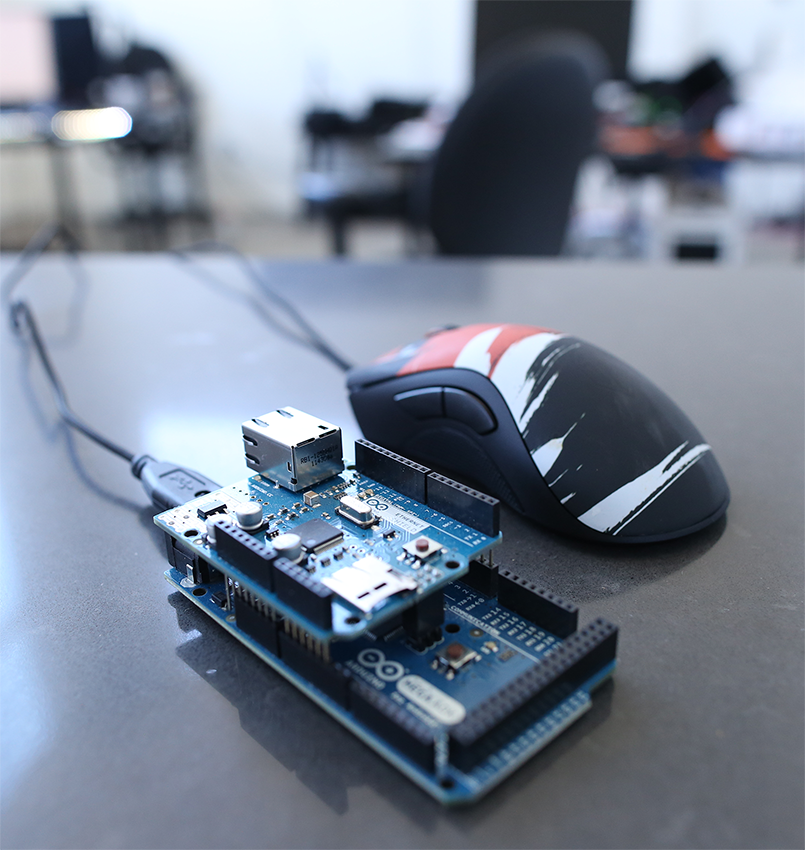
\includegraphics[width=7cm]{img/game-ref1}
\caption{De Game:ref, let op het arduino bordje en de netwerkpoort. Deze laatste is om contact te staan met de anti-cheat server.}
\end{figure}



\section{Sociale of Crowd-Sourced}
\label{sec:sociale}
Een van de laatste manieren om aan \gls{anti}ing te doen is via Sociale \gls{anti}s of ook wel ''Crowd-Sourced''. Dit zijn systemen die gebruikers laat kijken naar verdachte personen en hen laat beslissen of deze al dan niet valsspelen. 
\\

Hiermee zijn wel vier problemen:
\begin{enumerate}  
\item Eerst en vooral: hoe beslis je wie verdacht is en wie niet. Controleer je iedereen (willekeurige mensen via een steekproef) of laat je enkel aangeduide spelers gecontroleerd worden.
\item Ten tweede: wie laat je deze bekijken? Kan iedereen dit of zijn er toch vereisten zodat niet jan en alleman iemand kan veroordelen tot valsspelen. Want wat we ten zeerste willen vermijden zijn mensen die onrechtvaardig verbannen worden.
\item Als derde moeten we ook rekening houden met wanneer je beslist iemand te verbannen van je gameservers. Doen we dit wanneer er een iemand zegt dat deze valsspeelt op basis van 1 kijker? Of laten we meerdere mensen kijken en kijken we hoeveel procent van deze zegt dat de verdachte valsspeelt?
\item En als laatste: Hoe maak je dat mensen dit blijven doen en dit geen vergeten functie wordt? Geef je er iets voor in ruil of hoe houdt je mensen aangetrokken tot de functie.
\end{enumerate}

Dit wordt standaard wel al gedaan bij de laatste versie van Counter-Strike. Deze optie noemt ''Overwatch'' in het spel.
Hoe zij dit beschrijven is als volgt''The Overwatch lets the CS:GO community regulate itself by allowing qualified and experienced members of the community (‘investigators‘) to review reports of disruptive behavior, determine whether those reports are valid, and apply temporary bans if appropriate.'' \citep{overwatch}
\\

Hoe werkt dit nu precies? Mensen van een bepaalde rank binnen het spel en die een bepaald aantal spellen al gespeeld hebben krijgen toegang tot de functie. Eenmaal je dit hebt komt er in het start menu een knop waar je een ''Case kan reviewen''. Dit download dan een video bestand waar alle namen van spelers zijn uitgewist. De verdachte noemt ''The Suspect'' en je krijgt een videofragment te zien van een 10 tal rondes. Hierna sluit de video af en krijg je per \gls{cheat} categorie de optie om te kiezen of jij denkt of deze hier aan voldoet of niet. Deze case komt ook bij andere spelers terecht, wanneer een bepaald aantal bevestigd (het is onbekend hoeveel precies of procentueel) dan wordt ''The Suspect'' verbannen. Ze proberen je dit te doen aanhouden door je een melding te geven wanneer er iemand verbannen wordt die jij veroordeeld hebt. Op deze manier weten spelers dat ze de game zelf zo van \gls{cheat}ers proper houden en moet dit hen de neiging geven om dit vaker te doen.
\\

De beslissing wie verdacht is wordt genomen aan de hand van de spelers zelf. Als je een officiële match speelt kan je iemand rapporteren voor verdacht gedrag. Wanneer een bepaald aantal spelers dit doet komt deze terecht tussen de Overwatch cases.

\begin{figure}
\centering
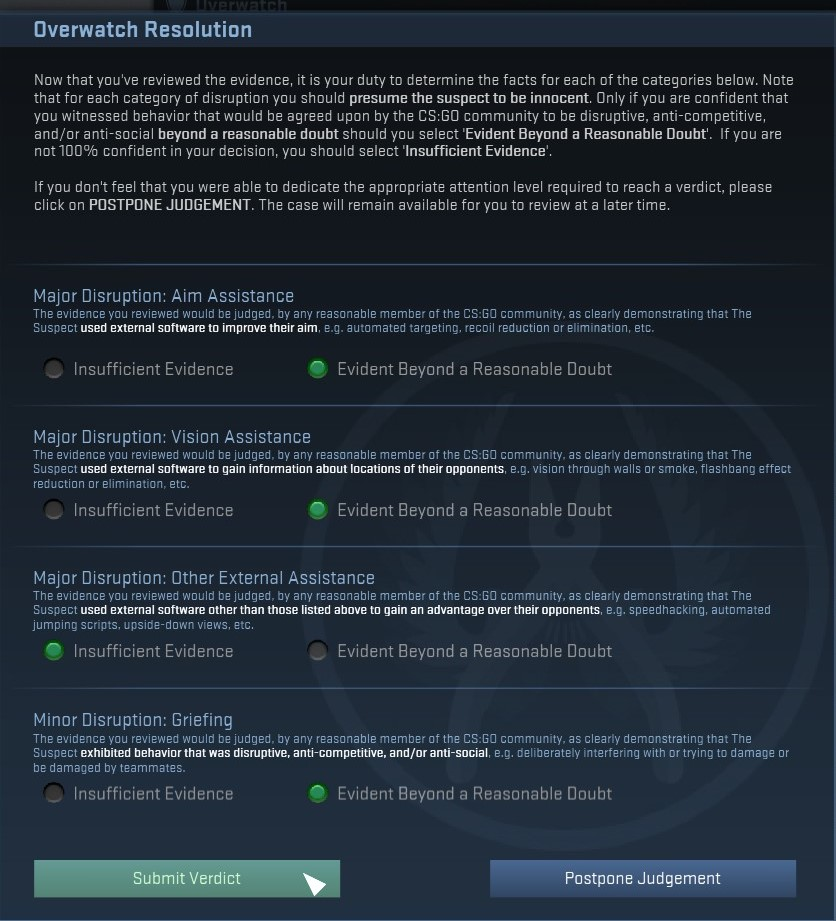
\includegraphics[width=7cm]{img/overwatch-example}
\caption{Een voorbeeld van de opties na het bekijken van een Overwatch video}
\end{figure}

\section{Banlists}
\label{sec:banlists}

Een andere interessante optie is het bannen van spelers aan de hand van het bijhouden van banlists. Hoe dit precies in zijn werk gaat is als volgt:
\begin{itemize}
\item Een speler beslist om vals te spelen op server A
\item De speler wordt gebanned van server A voor valsspelen (door een \gls{anti}).
\item De speler gaat naar server B (zonder vals te spelen)
\item Deze speler wordt ook van deze server verbannen omdat hij op de gekende lijst van valsspelers staat. 
\\
\end{itemize}


Hoe dit geïmplementeerd wordt hangt af van het platform. \gls{valve} heeft recent bijvoorbeeld iets nieuw geïntroduceerd die hierop aansluit. \gls{steam} (het platform waarop je games koopt en CS:GO onder draait, dit is ook ontwikkelt door \gls{valve}) heeft van vele gebruikers het GSM nummer staan. 
Dan kan je in game bevestigen dat je dit telefoonnummer wil koppelen aan je gameaccount. Dit levert voordelen op (die momenteel nog niet aangekondigd zijn op het moment van schrijven) voor de spelers. Het voordeel voor \gls{valve} is dan weer dat mensen die een account hebben die gebanned worden niet een nieuw account kunnen aanmaken met hetzelfde telefoonnummer. Anders zullen deze automatisch opnieuw gebanned worden. 

\section{Real life concept}
\label{sec:concept}
Voorgenoemde oplossing lijkt interessant te zijn met als toepassing een online platform zoals BeSports waar ik ervaring mee heb door mijn stage. 
Dit is een platform gemaakt voor Belgische gamers en iedereen kan hier aan deelnemen. Wanneer spelers meedoen met toernooien krijgen zij een prijs uitbetaald in een eigen munteenheid genaamd BeCoins.
Om hiermee producten te kopen moeten ze hun naam en adres in vullen.
\\

Als we een \gls{anti} hebben die 1) spelers banned als ze valsspelen en 2) rekening houdt met al bestaande verbannen gebruikers, kunnen we heel eenvoudig een setup maken die zo'n gebruikers van een online platform weghoudt. 
\\

Daarmee zou je dan een systeem kunnen ontwikkelen die wanneer iemand die gepakt word voor het valsspelen in een spel dit doorgegeven wordt aan het online platform. Hier kan deze persoon op een lijst geplaatst worden die het platform zelf onderhoud. Aan de hand daarvan kun je dan nagaan bij de creatie of wijziging van een speler of deze gelijke gegevens heeft als een verbannen gebruiker. Dit kan zijn zoals het hierboven vermeldde telefoonnummer maar dan ook het adres (die nodig is om prijzen uit te keren) en naam. Als er dus dan iemand een account maakt met zelfde gegevens zou je deze persoon automatisch toegang weer kunnen ontzeggen om zo terugkomende valsspelers permanent van het platform af te houden.
\\

Als deze gegevens dan nog eens naar een algemene database doorgestuurd worden die voor andere server beheerders ook beschikbaar is dan kan ieder platform zo heel eenvoudig een groot deel van de valsspelers weigeren. Dit kan voordeel hebben vergeleken met de ingebouwde \gls{anti} van \gls{valve} (\gls{vac}) omdat deze met vertraging werkt en het dus lang kan duren voor iemand officieel verbannen wordt.

\chapter{Uitvoeren van de test}
\label{ch:test}
Om de huidige situatie beter te snappen en te kijken wat de beste oplossing is heb ik een test opstelling gemaakt. Eerst en vooral werden er enkele \gls{cheat}s gedownload die voor een gewone gebruiker vrij eenvoudig te installeren zijn (vaak een gewoon .exe bestand). Deze werden dan getest op werking op een server die geen \gls{anti} had aanstaan. Eenmaal de werking bevestigd was werden deze apart gezet om ze nadien op een \gls{anti} los te laten.

\section{Opzetten van de gameserver}
\label{sec:gameserver}
Voor het opzetten van een gameserver is er gegaan voor het gebruik van Amazon Web Services. Omdat ik ervaring had opgedaan met dit leek het mij interessant om hier zo min mogelijk tijd aan te verliezen. Het voordeel was ook dat je dan echt duidelijk een server en een client hebt die een echte online situatie nabootsen. Daarna werd deze server opgestart met de optie ''-insecure'' dit zorgde ervoor dat de server geen standaard \gls{vac} draaide.
\\

Daarna werd \gls{smac} (SourceMod Anti-Cheat) gedownload. Dit was niet zo eenvoudig zoals het eerst leek. Voor dat dit werkende gekregen kon worden moest eerst Metamod:Source en Sourcemod geïnstalleerd worden. Dit zijn twee pakketen die samenwerken om dieper op server niveau in te spelen en het eenvoudiger maakt om plugins te schrijven.
Daarna kwam het probleem boven dat \gls{smac} niet vrij verkrijgbaar niet meer is. Hoewel het nog ontwikkeld wordt is de website offline gehaald zoals vooraf genoemd. Gelukkig had iemand een mirror opstaan die de laatste versie wel nog bevatte en konden we daar mee aan de slag. Via ftp werden alle plugins op de server geplaatst waarna de gameservice herstart werd. Wanneer je dan met de game verbond kon je direct merken dat \gls{smac} aanstond aan de hand van de melding ''This server is secured by \gls{smac}''. 
\\

Na het uitvoeren van het commando "smac\_status" krijg je bevestiging van de werking. Deze heeft een lijst van alle spelers terug die \gls{smac} herkent. Dus dan was het testen met de verschillende \gls{cheat}s.

\section{Uitvoeren test}
\label{sec:uitvoering}

Er werd gebruik gemaakt van een oude laptop die een grafische kaart ter beschikking had om het spel op een aanvaardbare manier te draaien (dus geen haperingen). Er werd dan via \gls{steam} een nieuwe kopie gekocht van \gls{csglobal}. Hierdoor is het zeker dat de tester niet op andere accounts schade heeft. Daarna werden de twee best werkende (aan de hand van tests ondervonden) \gls{cheat}s geïnstalleerd. Dit zijnde met naam ''ABitSmarter'' \citep{abitsmarter} en SE of ''Silent Evil'' \citep{silentevil}.
Beide zijn op het moment van schrijven nog niet gedetecteerd. Het valt wel op dat de eerst vernoemde wel iets groter is en is algemeen robuuster en gaat al vrij lang mee ook. Silent Evil is een \gls{cheat} die dan weer door een iemand ontwikkelt wordt en enkel publiekelijk beschikbaar is in tegenstelling tot ABitSmarter die ook een betalende versie heeft. 
\\

Na het connecteren met de server vanuit het spel werden voor elk eens de \gls{cheat} geactiveerd en getest. Beiden werkten vrij goed en gaven een heel duidelijk voordeel. De tweede was een heel stuk opvallender dan de eerste voor buitenstaanders. De eerste moest je zelf nog ongeveer mikken maar nam over bij het mikken zodra je in de buurt van iemand kwam.
\\

Er werd uitvoerig getest met deze twee tools om de speler te helpen. Het viel heel hard op hoe eenvoudig het wel niet is om aan dergelijke praktijken mee te doen. Het verwonderde mij ook hoe subtiel het soms wel kon zijn, het hangt heel hard af van de speler hoe goed deze het wil verbergen voor mensen die zouden meekijken zoals bijvoorbeeld bovenvermelde Overwatch kijkers.

\begin{figure}
\centering
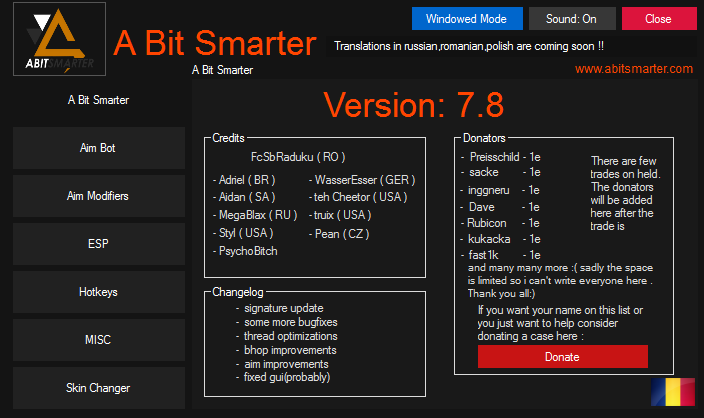
\includegraphics[width=12cm]{img/abitsmarter}
\caption{De GUI van A Bit Smarter, dit is vrij eenvoudig in gebruik en je ziet ook alle opties onder categorieën.}
\end{figure}
\begin{figure}
\centering
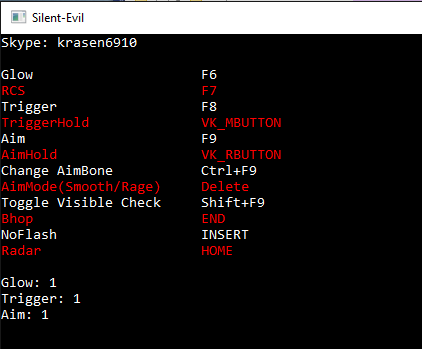
\includegraphics[width=8cm]{img/silentevil}
\caption{De CLI van Silent Evil (heel standaard maar doet wat het moet doen).}
\end{figure}


\section{Resultaten}
\label{sec:resultaten}
De resultaten waren helemaal niet zoals eerst verwacht. Na deze beide getest te hebben werd er terug naar de server gegaan om te kijken naar de \gls{anti} logs (dit is waar ieder verdachte beweging wordt geregistreerd met details over welke speler het gaat en welke overtreding het zou zijn). Hier stond geen enkele overtreding in en beide \gls{cheat}s werden niet gedetecteerd. Dit is een van de meest gebruikte \gls{anti}s en momenteel de enige die zelf te installeren valt zonder een hoge kost. 
\\

Dus mijn volgend idee was om de standaard \gls{anti} aan te zetten om te kijken wat mogelijk was te \gls{cheat}en op een dubbel beveiligd server. \gls{vac} heeft wat tijd nodig om een ban uit te leveren (dit is zo waardoor het niet mogelijk is voor mensen om te weten door welke \gls{cheat} ze gebanned als ze meerdere proberen). Maar na een eind te testen zelf online tegen andere spelers was voor hen het vrij duidelijk dat de er vals gespeeld werd maar er werd niets aan gedaan door \gls{vac}.
\\

Er werden meerdere spellen gespeeld terwijl er heel duidelijk vals gespeeld werd op momenten maar geen enkele \gls{anti} software heeft deze gedetecteerd. Dit heeft heeft een goed beeld van de huidige situatie van computergames en meer bepaald \gls{esports}. \Gls{cheat}en is mogelijk en het is heel moeilijk om de personen tegen te houden.

\chapter{Mening van een anti-cheat ontwikkelaar}
\label{ch:mening}
Zoals in het vorige hoofdstuk al opvalt is dat het heel moeilijk is om mensen die zin hebben om vals te spelen tegen te gaan. Een goed beeld krijgen van de huidige situatie als buitenstaander is dan ook heel moeilijk, zelf voor een speler die er dagelijks mee bezig is kan het moeilijk zijn om een idee te hebben wat er zich allemaal afspeelt onder de \gls{cheat}ers en \gls{anti} ontwikkelaars. 
\\

Hier rond heeft de gebruiker 'debuglog' onlangs een uitgebreide mening over geschreven. Deze persoon heeft 7 jaar ervaring in het ontwikkelen van \gls{cheat}s en twee jaar met het maken van \gls{anti}s. Ook houdt hij een persoonlijke blog bij waar hij meerdere aspecten van \gls{anti}s bespreekt binnen Counter-Strike. Samen met posts die andere \gls{anti} methodes op een kritische manier bekijkt.\citep{debuglogblog}
\\

Wat heel duidelijk wordt uit zijn statement is dat er momenteel heel wat \gls{cheat}ers zijn en dat het heel moeilijk is om een goeie \gls{anti} te schrijven. Vaak zijn er heel wat beperkende factoren die het tegengaan van deze valsspelers bemoeilijkt. 
\\

Een van de hoofdredenen die het zoeken naar \gls{cheat}s tegenhoudt is de computer van de gebruiker. Vaak is deze volop in gebruik door de game die momenteel gespeeld wordt. Hierdoor is het bijna niet mogelijk om op een snelle manier informatie te verzamelen zonder de gameplay te beïnvloeden. Heel veel mensen hebben last van haperingen en \gls{lag} wanneer ze gebruik maken van een iets diepgaandere \gls{anti}.
Dit zou geen probleem zijn moesten de cheats niet zo geavanceerd zijn. Maar het is moeilijk om een heel diepgaande scan uit te voeren die toch snel is en geen opstopping wordt voor de computer van de gebruiker, dus een vervelende limitatie. 
\\

Daarbovenop komt dan ook nog eens dat als het mogelijk zou zijn om een \gls{anti} te ontwikkelen die goed genoeg is om heel snel alle bestanden te scannen zonder dat het systeem er onder lijdt er nog altijd problemen zouden zijn. Het is namelijk volgens de wet gereguleerd dat niet alle bestanden mogen doorzocht worden van de potentiële valsspelers. Dus naast de systemen is dit ook een grote drempel die het maken van goede preventiesystemen tegengaat.
\\

Wat hij ook vermeld is dat valsspelers er vaak veel aan zullen doen om van de \gls{anti} af te raken. Hiervoor is het dus nodig dat je het systeem ook goed genoeg beschermd maakt tegen die gebruikers die er net iets meer moeite voor doen om niet gepakt te worden. Dan is het de afweging maken tussen het systeem robuust maken of het systeem beter te optimaliseren.
\\

Naast deze elementen is het dan nog eens heel moeilijk om geen enkele fout te maken, je wil namelijk niet dat iemand onschuldig bestraft zal worden. Mensen betalen nog altijd voor het spel en spelen dit vaak voor hun plezier, dan is het jammer als dit wordt weggenomen voor iemand die gewoon met zijn vrienden aan het spelen was. Het kan ook zeer negatieve reclame zijn als dit voorkomt. Het probleem is dat een programma vaak moeilijkheden heeft om te beslissen wat nu nog net wel mogelijk is en wat door een \gls{cheat} uitgevoerd wordt. Je wil ook niet dat er twijfel komt over de correctheid van het \gls{anti} systeem, de gebruikers moeten er in geloven zodat ze een reden hebben om te blijven spelen op jou platform.
\\

Voorgaande problemen zijn nog maar het begin om het zo te zeggen. Een principe die al heel lang meegaat binnen het ontwikkelen van \gls{cheat} is zoals hij het noemt "first one to load wins". Dit houdt in dat ieder programma die eerst gestart wordt volgende programma's die gestart worden kan beheren. Dit is iets dat ik vaak merkte bij het opstarten van een \gls{cheat}: eerst de \gls{cheat} zelf opstarten en dan vroeg hij om de game op te starten.
\\

Hiermee zouden mensen zoals hij het noemt een bijna ondetecteerbare \gls{cheat} kunnen maken als het goed uitgewerkt wordt. Als er iemand het idee heeft om iets te schrijven die inlaadt voor het besturingssysteem dan kan deze alles besturen en aanpassen én zou het nog eens zo goed als onmogelijk zijn om op gelijk welke manier te bepalen of het een \gls{cheat} is of niet. Hij vermeld er wel bij dat dit waarschijnlijk nog niet bestaat of enkel op heel kleine schaal omdat het voor de \gls{cheat} ontwikkelaar een heel moeilijk proces is om zo'n \gls{cheat} stabiel en veilig te maken.
\\

Als laatste legt hij nog uit wat het probleem met herwerkte code zoals met een poly\gls{cheat} die hierboven vermeld staat. Deze verbergen de werkelijke code om scans buiten spel te plaatsen. Als we dit vergelijken met hoe anti-virus dit oplost: neem een emulator die de code uitvoert in een gesloten omgeving, moeten we weer ingeven op het feit dat de beschikbare computer resources beperkt zijn. Het is niet mogelijk om alle verdachte code in een gesloten omgeving uit te voeren zonder van de game-ervaring weg te nemen. Het is ook een heel stuk eenvoudiger om code te verbergen dan om ze terug tevoorschijn te toveren. Dit heeft de \gls{cheat} ontwikkelaars het voordeel in de meeste situaties.
\\

Als besluit komt hier dan uit dat iemand die iets kent van het ontwikkelen van \gls{cheat}s vaak het voordeel heeft van de twijfel. Als alles blijft verder gaan aan de huidige trend zou de \gls{anti} de strijd verliezen. 
\\

We kunnen enkel maar hopen dat er plotse vooruitgang wordt geboekt op het vlak van \gls{anti}s en nog liefst met de ingebouwde \gls{valve} Anti-Cheat. Want als de trend zich verder zet zal het natuurlijk ongeloofwaardiger worden wanneer er professionele spelers een merkwaardige prestatie neerzetten. 
\citep{debuglog}

\chapter{Conclusie}
\label{ch:conclusie}

% TODO: Trek een duidelijke conclusie, in de vorm van een antwoord op de
% onderzoeksvra(a)g(en). Reflecteer kritisch over het resultaat. Zijn er
% zaken die nog niet duidelijk zijn? Heeft het ondezoek geleid tot nieuwe
% vragen die uitnodigen tot verder onderzoek?
Het onderzoek ging omtrent de beste methode van het tegengaan van valsspeler in online games meer bepaald \gls{fpsgames}. Er werd eerst diep onderzoek gedaan naar de mogelijkheden voor de valsspelers en wat zij zoal tegenkomen. Daar valt op dat er een zee aan mogelijkheden is waarvan er maar enkele getest zijn in dit onderzoek. Ook zijn er waarschijnlijk nog heel wat geavanceerdere \gls{cheat}s die niet de revue gepasseerd zijn dus die nog minder snel gedetecteerd zouden worden, het is nog maar het topje van de ijsberg.
\\

Hoewel het moeilijk is om na te gaan is hoeveel mensen er nu werkelijk valsspelen valt het heel hard op dat in standaard modus er heel veel valsspelers meedoen. Het is zelf zo erg dat deze geautomatiseerd promotie maken voor de site vanwaar ze deze gehaald hebben in de chat.
\\

Hoewel het spel dus gigantisch populair is onder de kijkers in de \gls{esports} wereld moet er dus wel iets gedaan worden om het spel nog zijn waardigheid te doen houden. Er zijn zoveel toffe aspecten aan het spel maar dit wordt overschaduwd door de mensen die dit proberen weg te nemen.
\\

Momenteel is het advies voor een online platform toch wel dat er best gebruik gemaakt wordt van \gls{smac}. Hoewel het in mijn test niet goed genoeg was zal het wel nog enkele slechtere \gls{cheat}s er van tussen nemen. Het voordeel hieraan is dat je heel eenvoudig ook mensen kunt bannen die op andere services ook de toegang ontzegt zijn (waar vaak een diepgaandere \gls{anti} aanwezig is). Ook zal het wel afschrikken als spelers zien bij het deelnemen aan een spel dat er gecontroleerd wordt met Sourcemod Anti-Cheat. 
\newpage 

Uiteindelijk denk ik dat bedrijven die iets serieuzer genomen willen worden best kijken naar de ontwikkeling van een eigen \gls{anti} die iets diepgaander is waarbij er ook van de speler uit verwacht wordt dat deze een client installeren. Het voordeel hiervan is dat er veel diepgaander kan gekeken worden op de speler zijn computer. Hiermee moet er wel nauw gelet worden op de wetgeving hierover.

\bibliographystyle{apa}
\bibliography{tin-bachproef}

%%---------- Back matter -------------------------------------------------

\listoffigures
%\listoftables

\end{document}
